\documentclass[color=usenames,dvipsnames]{beamer}\usepackage[]{graphicx}\usepackage[]{color}
% maxwidth is the original width if it is less than linewidth
% otherwise use linewidth (to make sure the graphics do not exceed the margin)
\makeatletter
\def\maxwidth{ %
  \ifdim\Gin@nat@width>\linewidth
    \linewidth
  \else
    \Gin@nat@width
  \fi
}
\makeatother

\definecolor{fgcolor}{rgb}{0, 0, 0}
\newcommand{\hlnum}[1]{\textcolor[rgb]{0.69,0.494,0}{#1}}%
\newcommand{\hlstr}[1]{\textcolor[rgb]{0.749,0.012,0.012}{#1}}%
\newcommand{\hlcom}[1]{\textcolor[rgb]{0.514,0.506,0.514}{\textit{#1}}}%
\newcommand{\hlopt}[1]{\textcolor[rgb]{0,0,0}{#1}}%
\newcommand{\hlstd}[1]{\textcolor[rgb]{0,0,0}{#1}}%
\newcommand{\hlkwa}[1]{\textcolor[rgb]{0,0,0}{\textbf{#1}}}%
\newcommand{\hlkwb}[1]{\textcolor[rgb]{0,0.341,0.682}{#1}}%
\newcommand{\hlkwc}[1]{\textcolor[rgb]{0,0,0}{\textbf{#1}}}%
\newcommand{\hlkwd}[1]{\textcolor[rgb]{0.004,0.004,0.506}{#1}}%
\let\hlipl\hlkwb

\usepackage{framed}
\makeatletter
\newenvironment{kframe}{%
 \def\at@end@of@kframe{}%
 \ifinner\ifhmode%
  \def\at@end@of@kframe{\end{minipage}}%
  \begin{minipage}{\columnwidth}%
 \fi\fi%
 \def\FrameCommand##1{\hskip\@totalleftmargin \hskip-\fboxsep
 \colorbox{shadecolor}{##1}\hskip-\fboxsep
     % There is no \\@totalrightmargin, so:
     \hskip-\linewidth \hskip-\@totalleftmargin \hskip\columnwidth}%
 \MakeFramed {\advance\hsize-\width
   \@totalleftmargin\z@ \linewidth\hsize
   \@setminipage}}%
 {\par\unskip\endMakeFramed%
 \at@end@of@kframe}
\makeatother

\definecolor{shadecolor}{rgb}{.97, .97, .97}
\definecolor{messagecolor}{rgb}{0, 0, 0}
\definecolor{warningcolor}{rgb}{1, 0, 1}
\definecolor{errorcolor}{rgb}{1, 0, 0}
\newenvironment{knitrout}{}{} % an empty environment to be redefined in TeX

\usepackage{alltt}
%\documentclass[color=usenames,dvipsnames,handout]{beamer}

%\usepackage[roman]{../pres1}
\usepackage[sans]{../pres1}






%% New command for inline code that isn't to be evaluated
\definecolor{inlinecolor}{rgb}{0.878, 0.918, 0.933}       % edit-kwrite
%\definecolor{inlinecolor}{rgb}{0.97, 0.97, 0.97}           % acid
\newcommand{\inr}[1]{\colorbox{inlinecolor}{\texttt{#1}}}

%\fboxsep=0mm
\IfFileExists{upquote.sty}{\usepackage{upquote}}{}
\begin{document}


\begin{frame}[plain]
  \huge
  \begin{center}
    \huge Applied Population Dynamics \\
    \LARGE Lab 1 -- Excel and R Basics \\
%    \large January 14 \& 18, 2019 \par
    \vspace{.5cm}
    \fbox{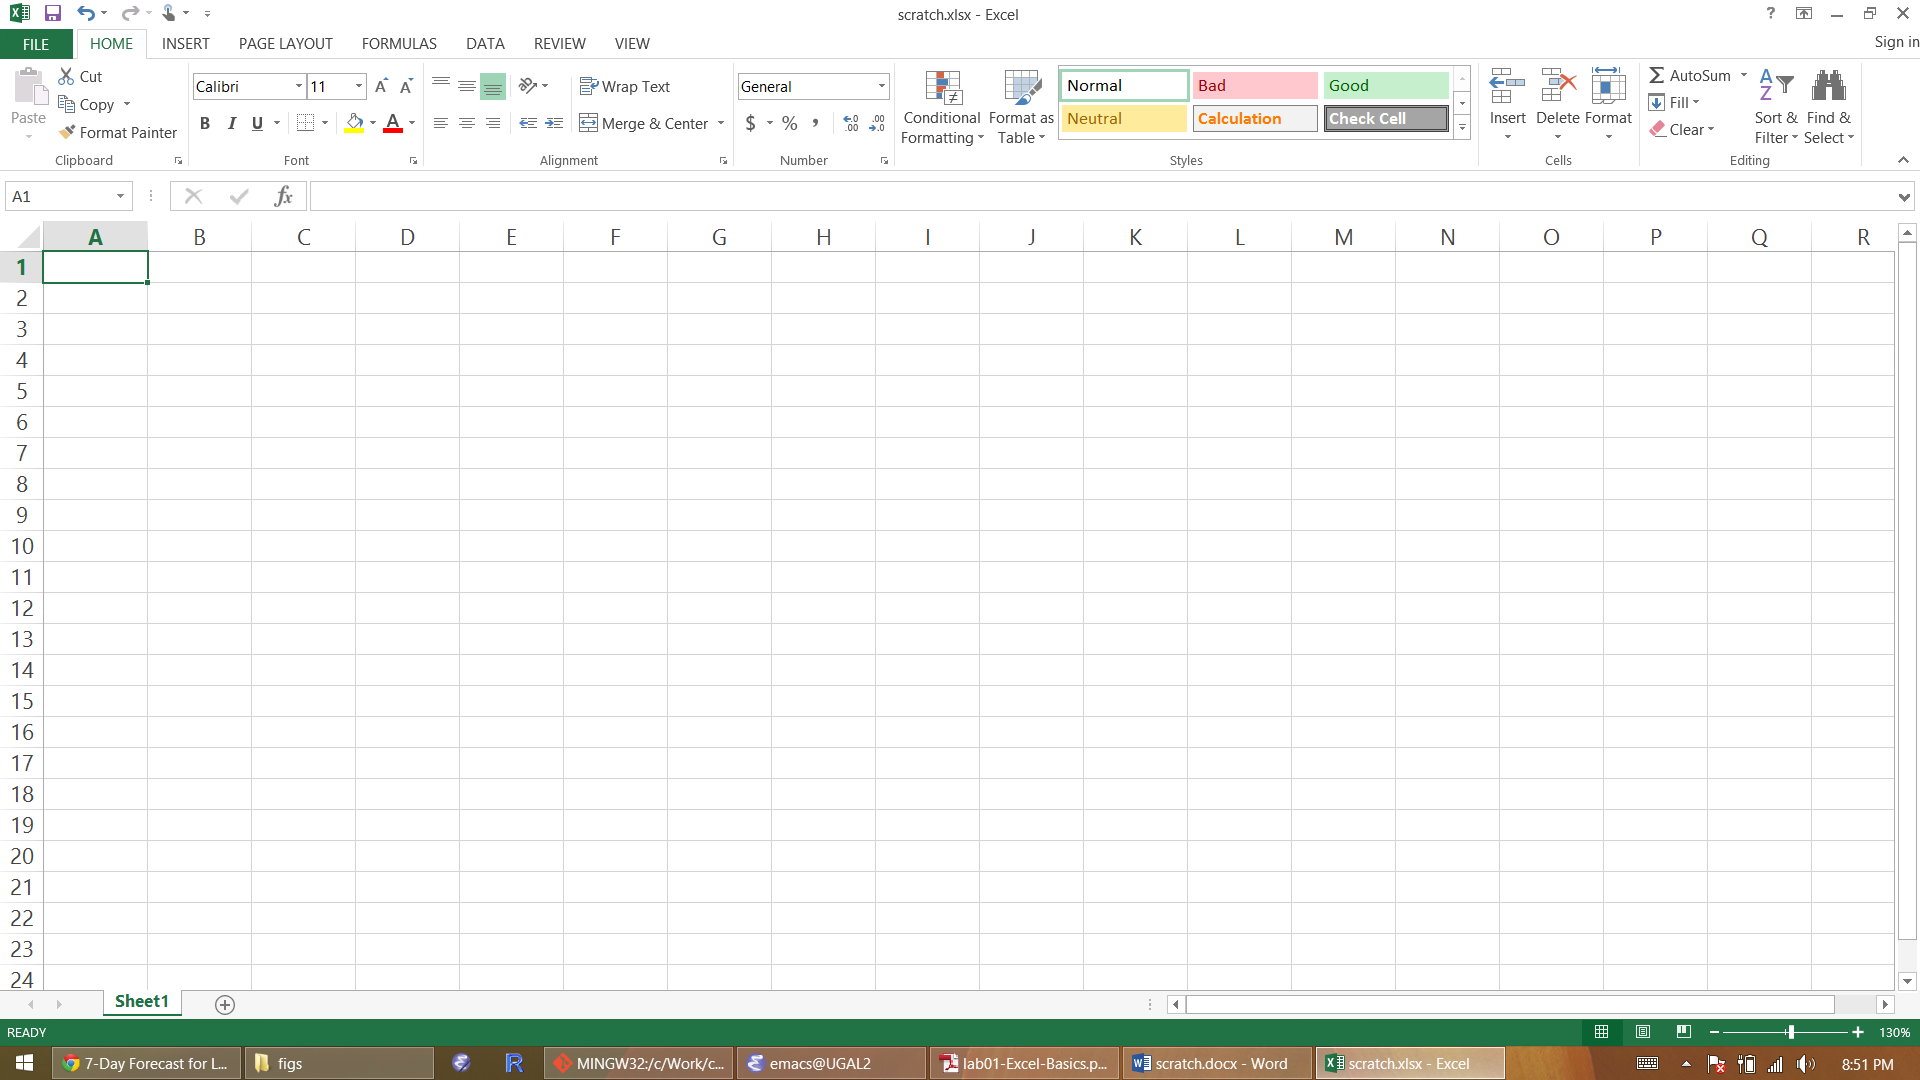
\includegraphics[width=\textwidth]{figs/excel}}
  \end{center}
\end{frame}


\section{Referencing}


\begin{frame}
  \frametitle{Column B}
  \fbox{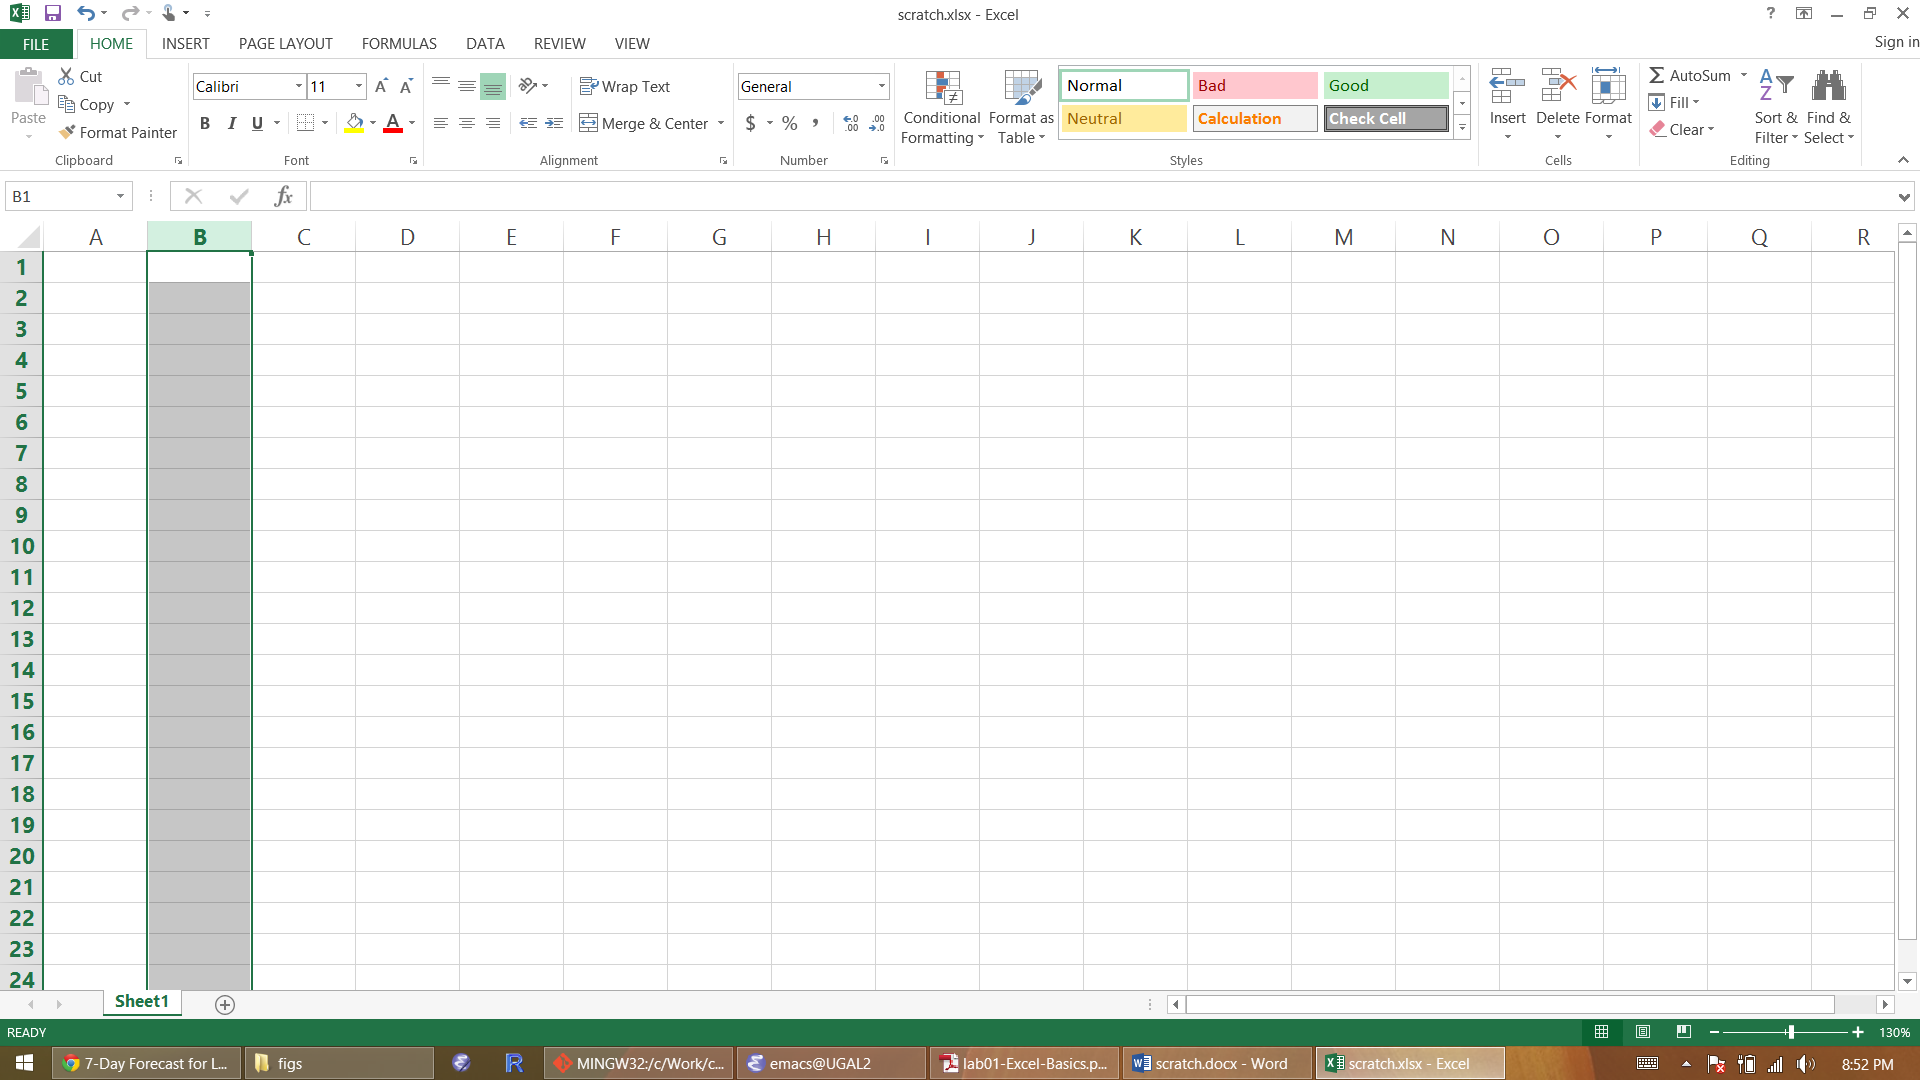
\includegraphics[width=\textwidth]{figs/columnB}}
\end{frame}


\begin{frame}
  \frametitle{Row 3}
  \fbox{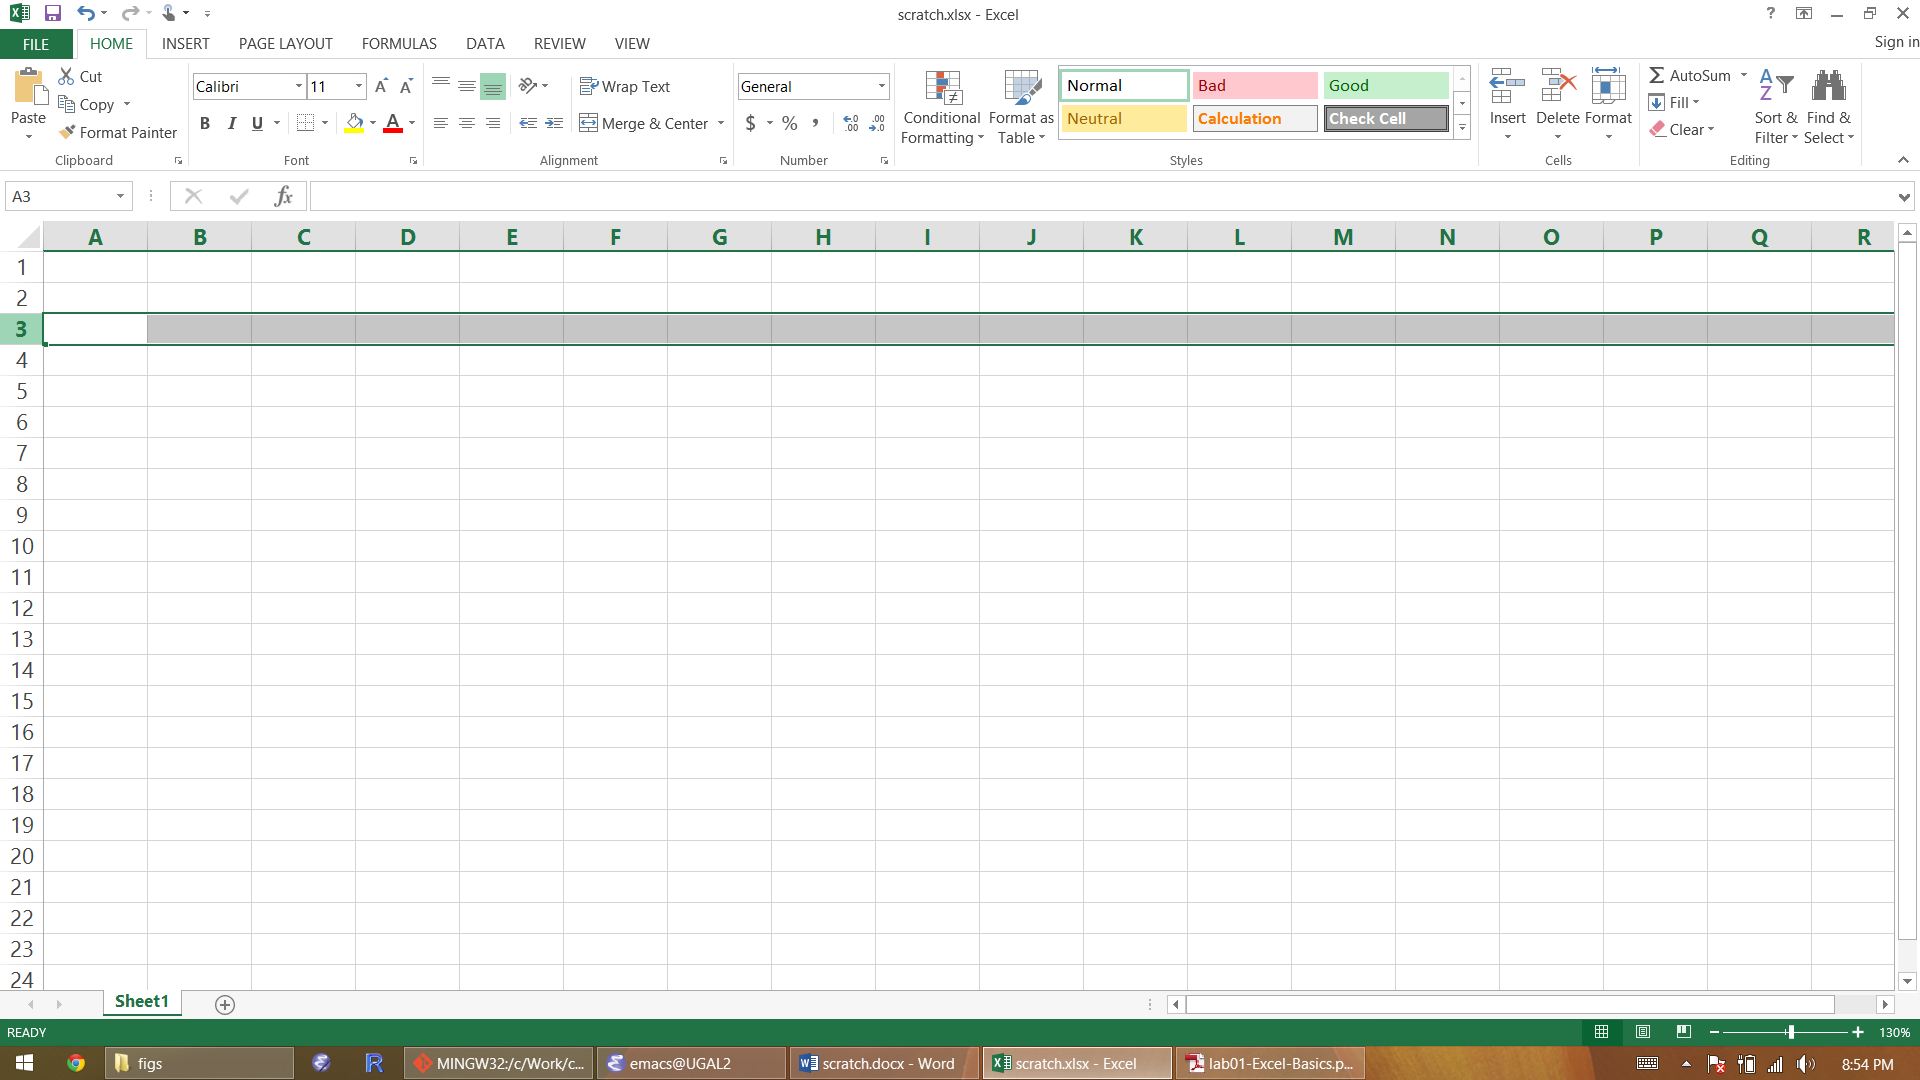
\includegraphics[width=\textwidth]{figs/row3}}
\end{frame}



\begin{frame}
  \frametitle{Cell B3}
  \fbox{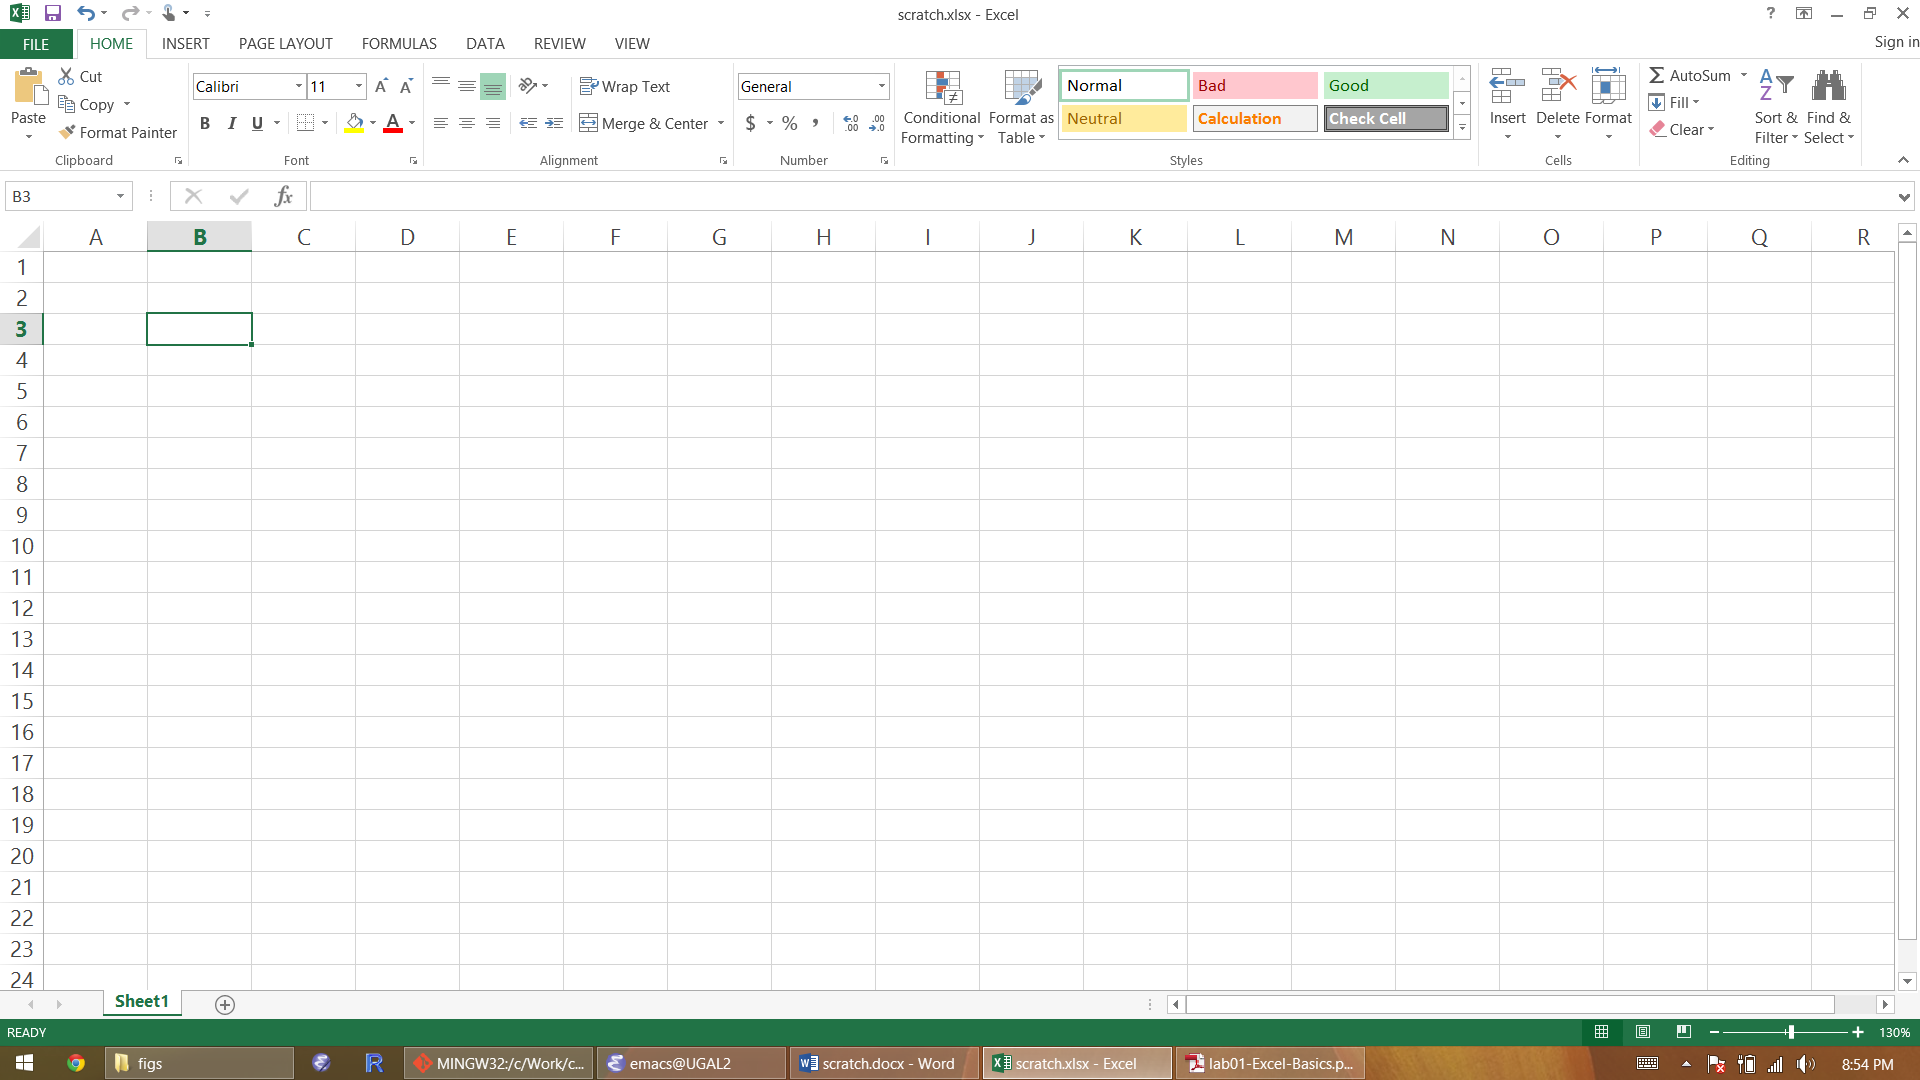
\includegraphics[width=\textwidth]{figs/cellB3}}
\end{frame}



\begin{frame}
  \frametitle{Create Sequence Using Auto-fill}
  \fbox{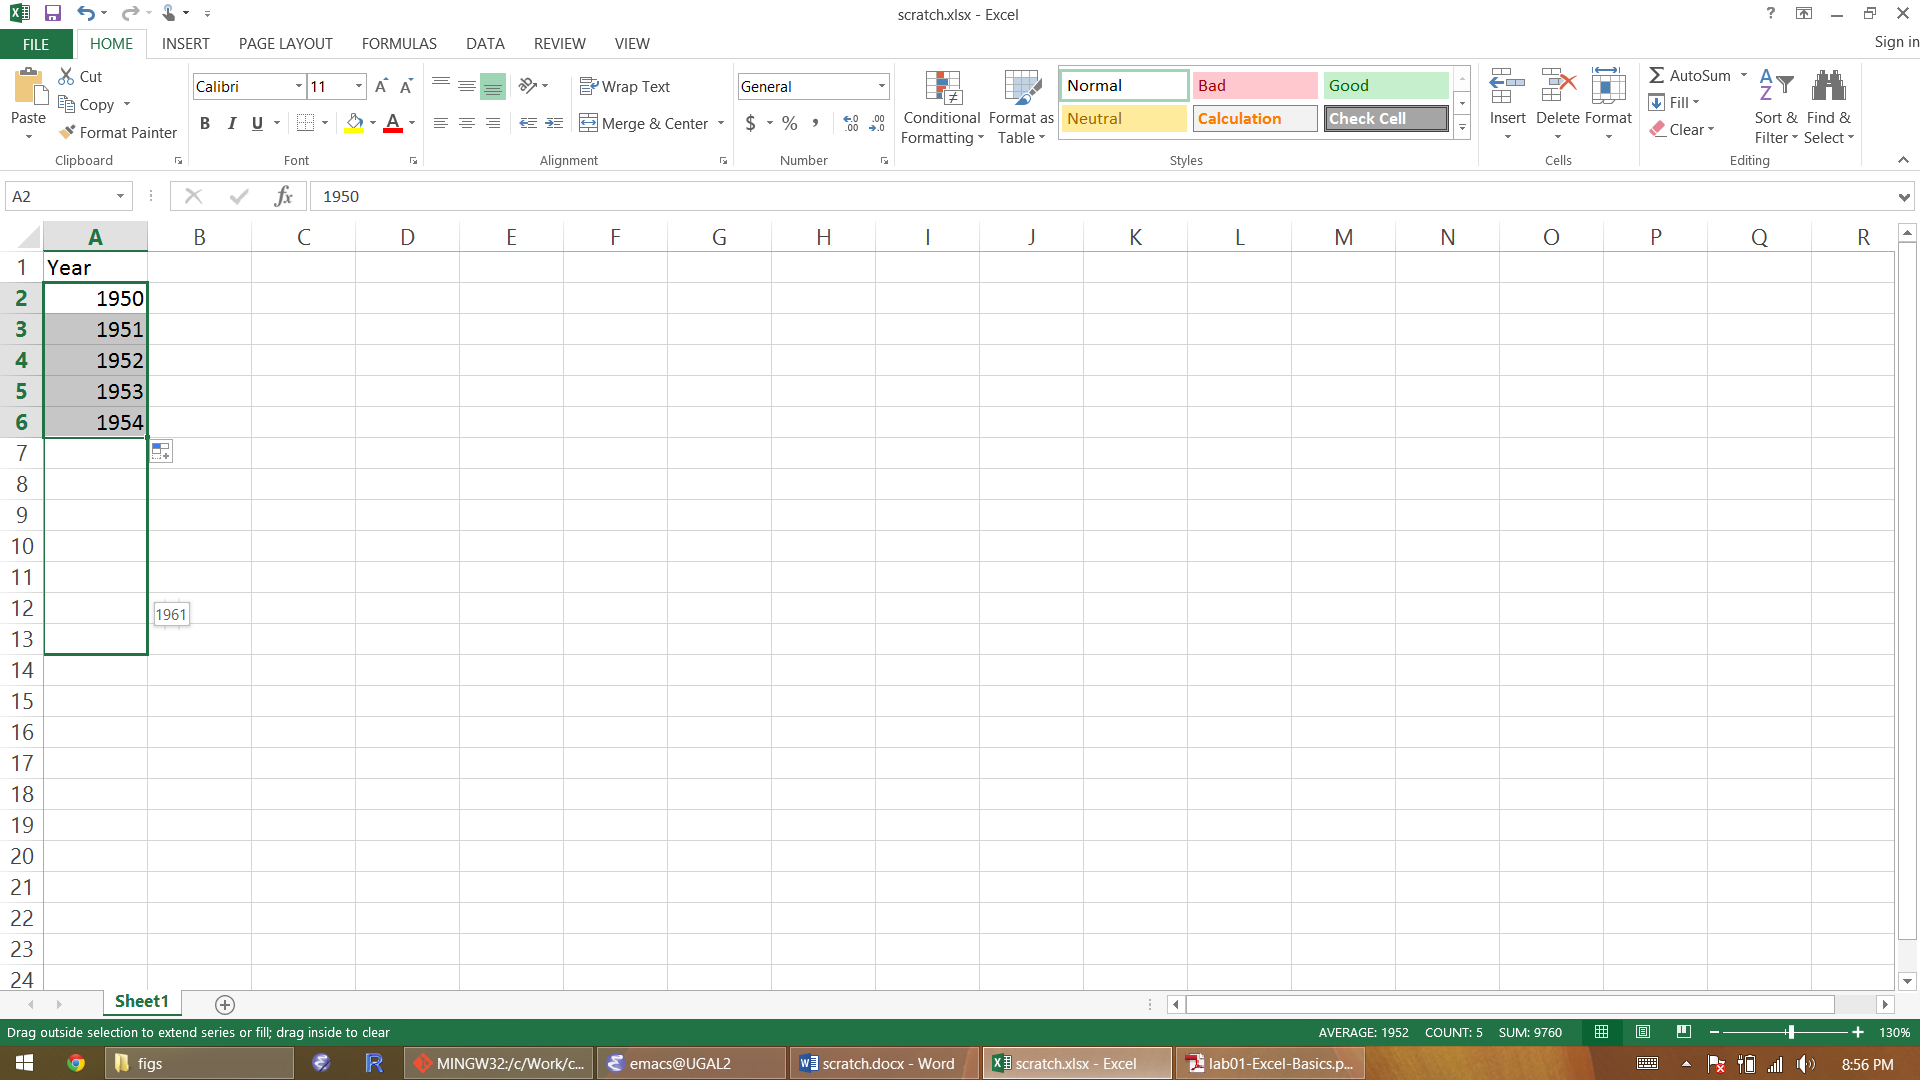
\includegraphics[width=\textwidth]{figs/sequence}} \\
  \centering
  To use auto-fill: begin a sequence, highlight the cells, and then
  drag the box at the bottom-right of the last cell. \\
\end{frame}


\begin{frame}
  \frametitle{Relative Cell References}
  \only<1>{\fbox{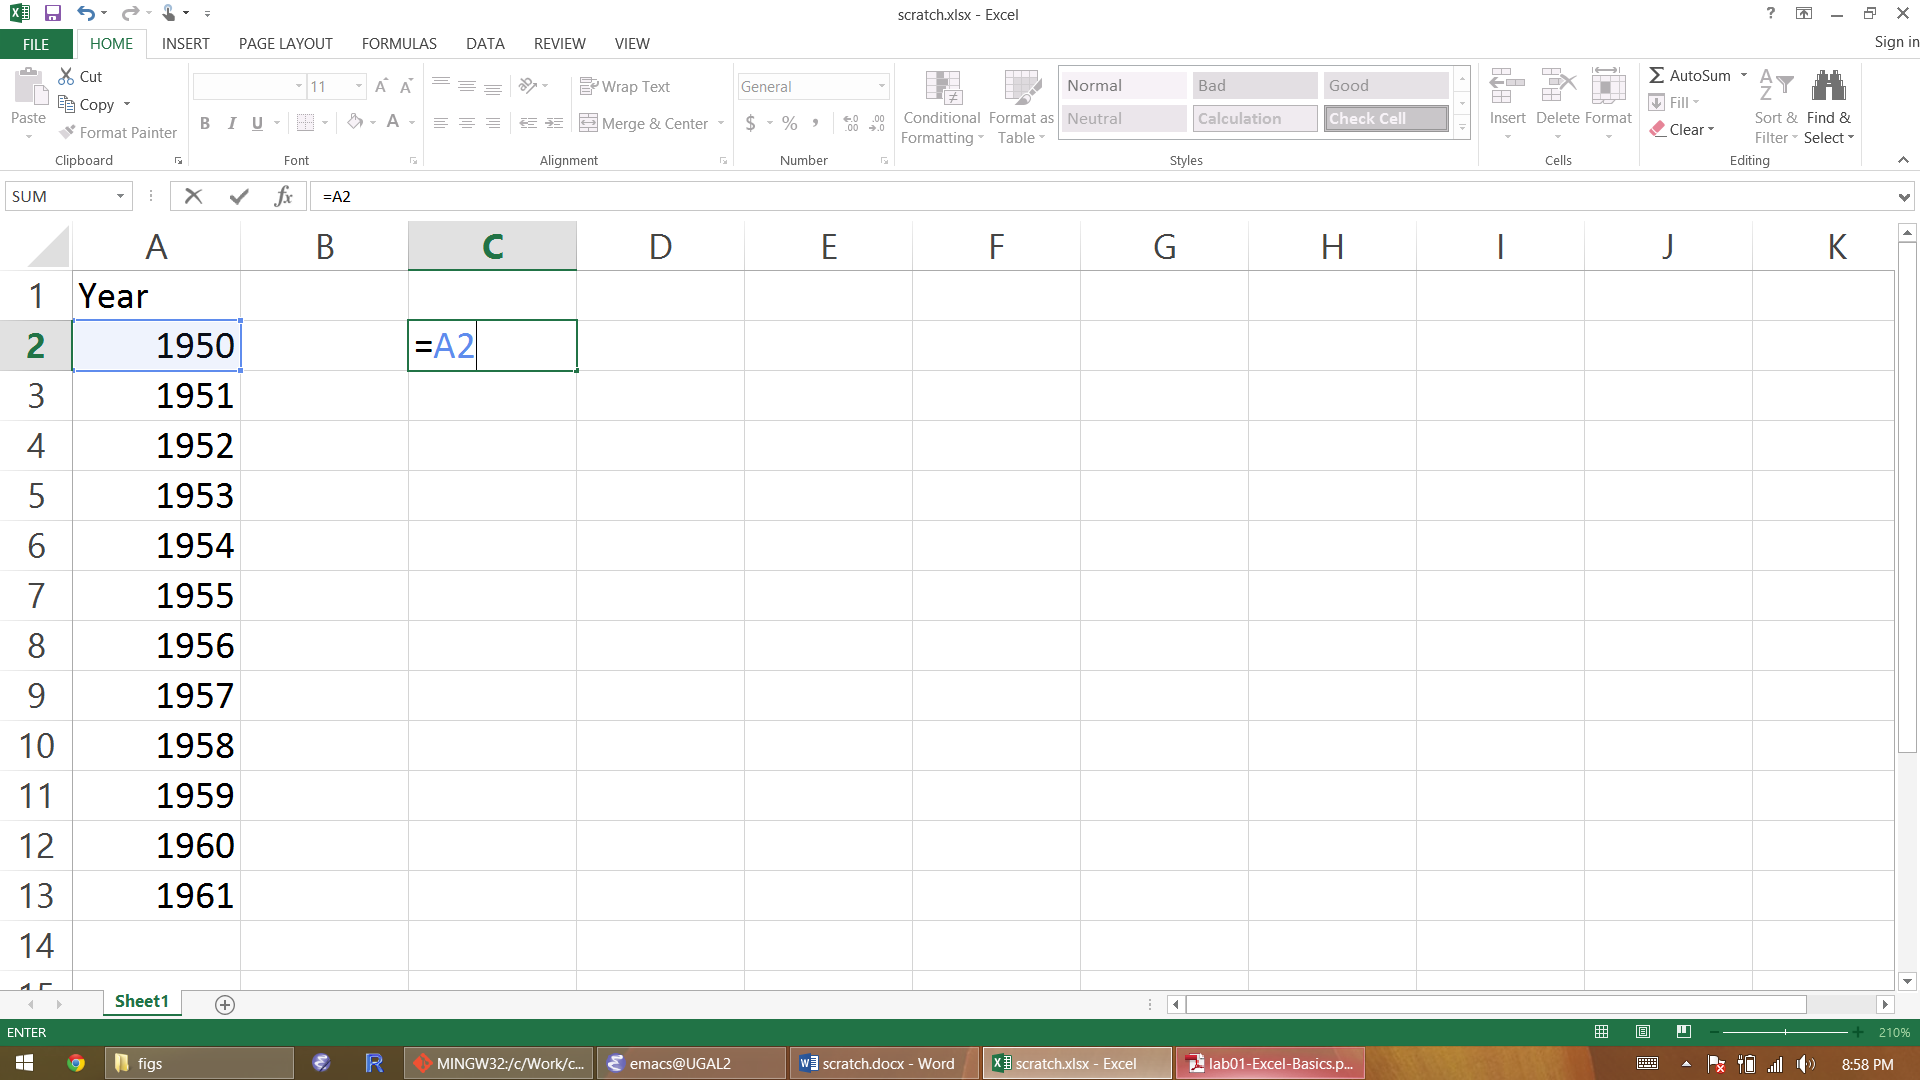
\includegraphics[width=\textwidth]{figs/relative-ref}}}
  \only<2 | handout:0>{\fbox{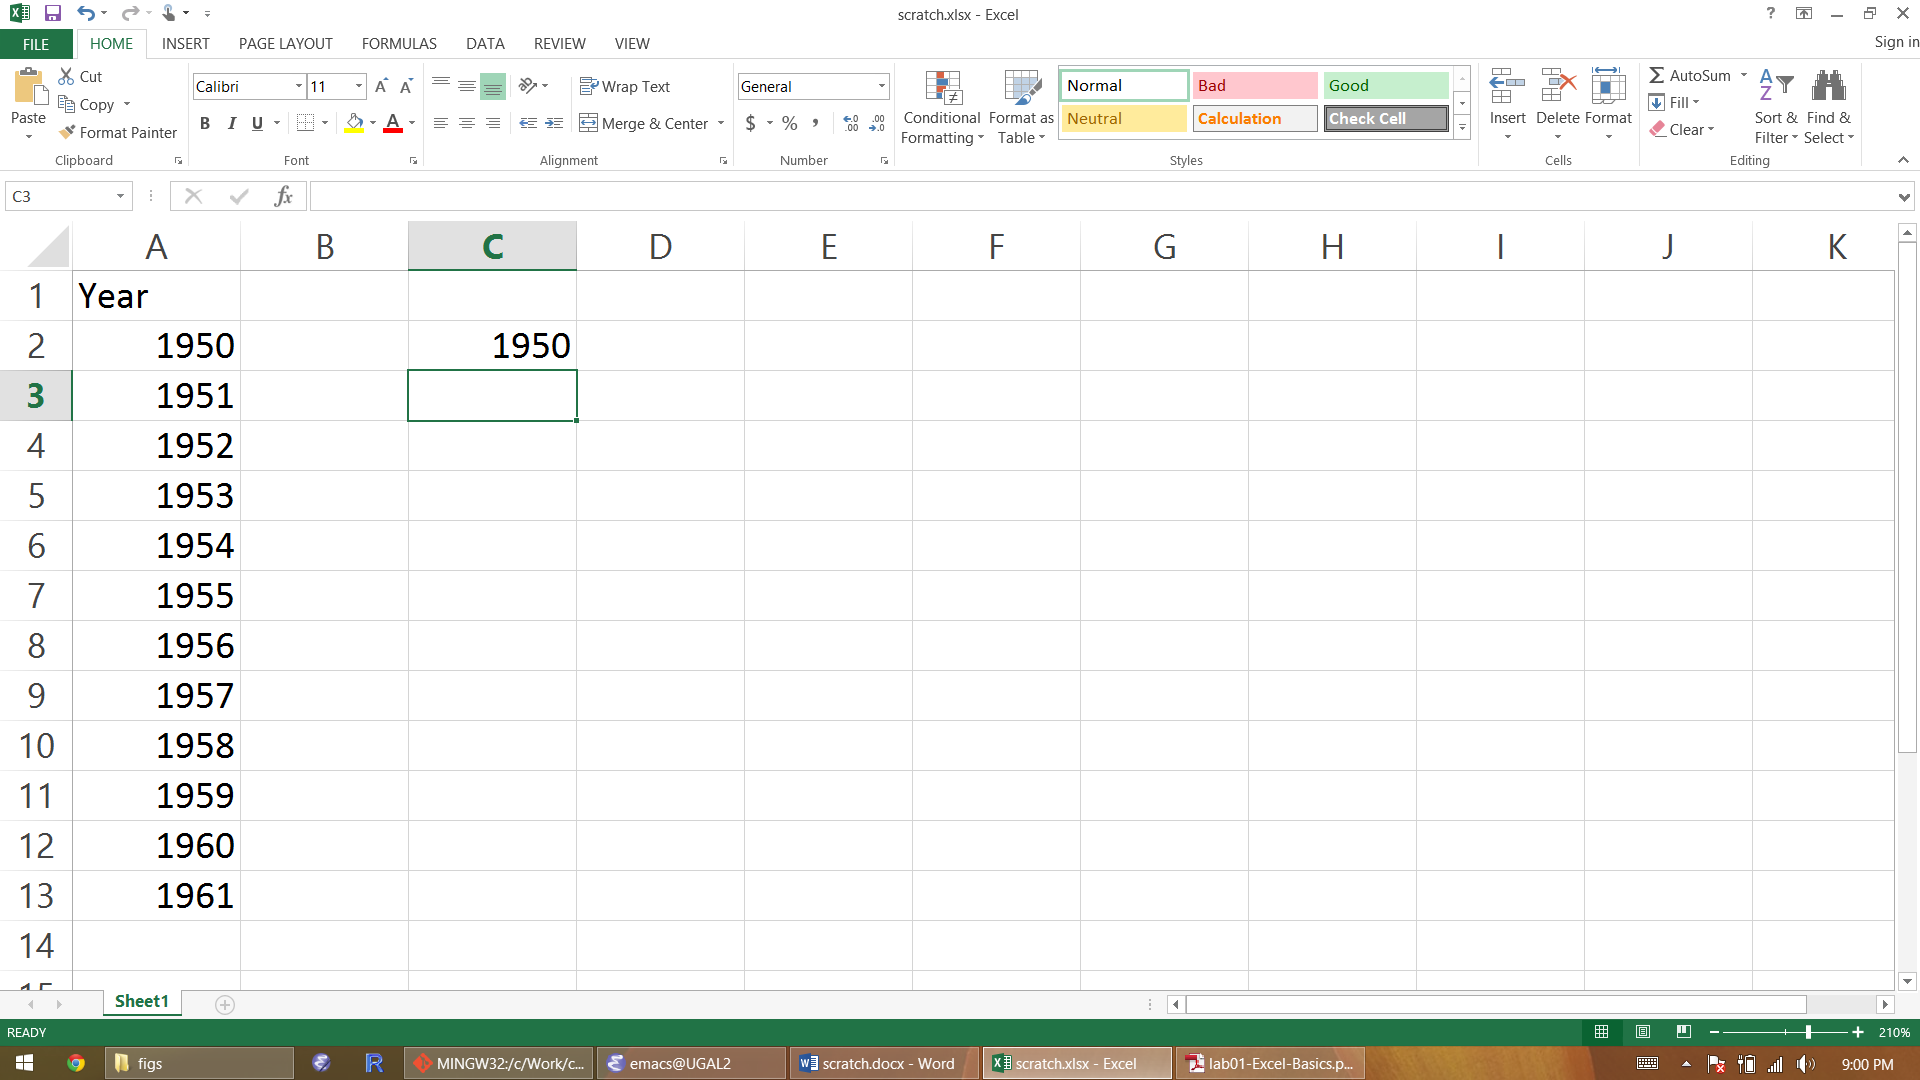
\includegraphics[width=\textwidth]{figs/relative-ref2}}}
  \begin{center}
    Cell C2 will take on the value of A2
  \end{center}
\end{frame}


\begin{frame}
  \frametitle{Relative Cell References}
  \fbox{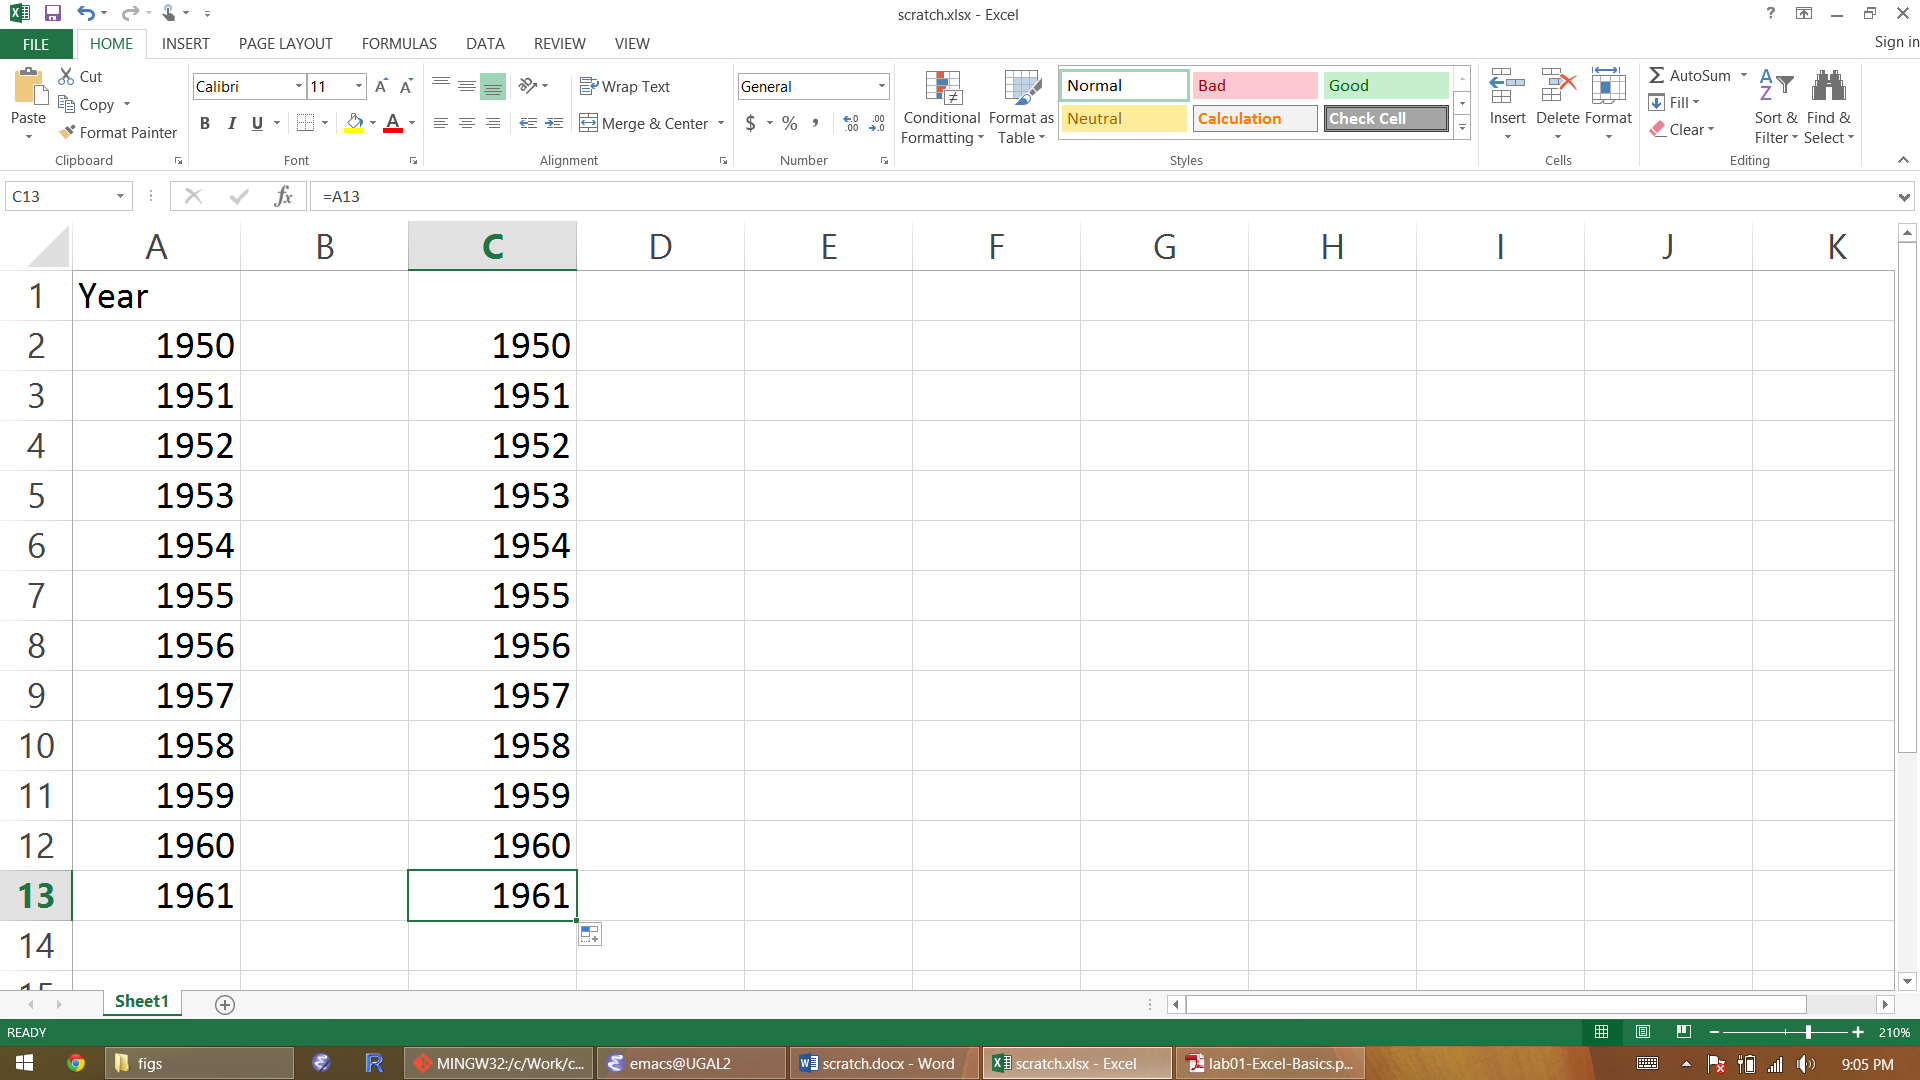
\includegraphics[width=\textwidth]{figs/relative-ref3}}
  \begin{center}
    Values of reference will change when using auto-fill
  \end{center}
\end{frame}


\begin{frame}
  \frametitle{Absolute Cell References}
  \only<1>{\fbox{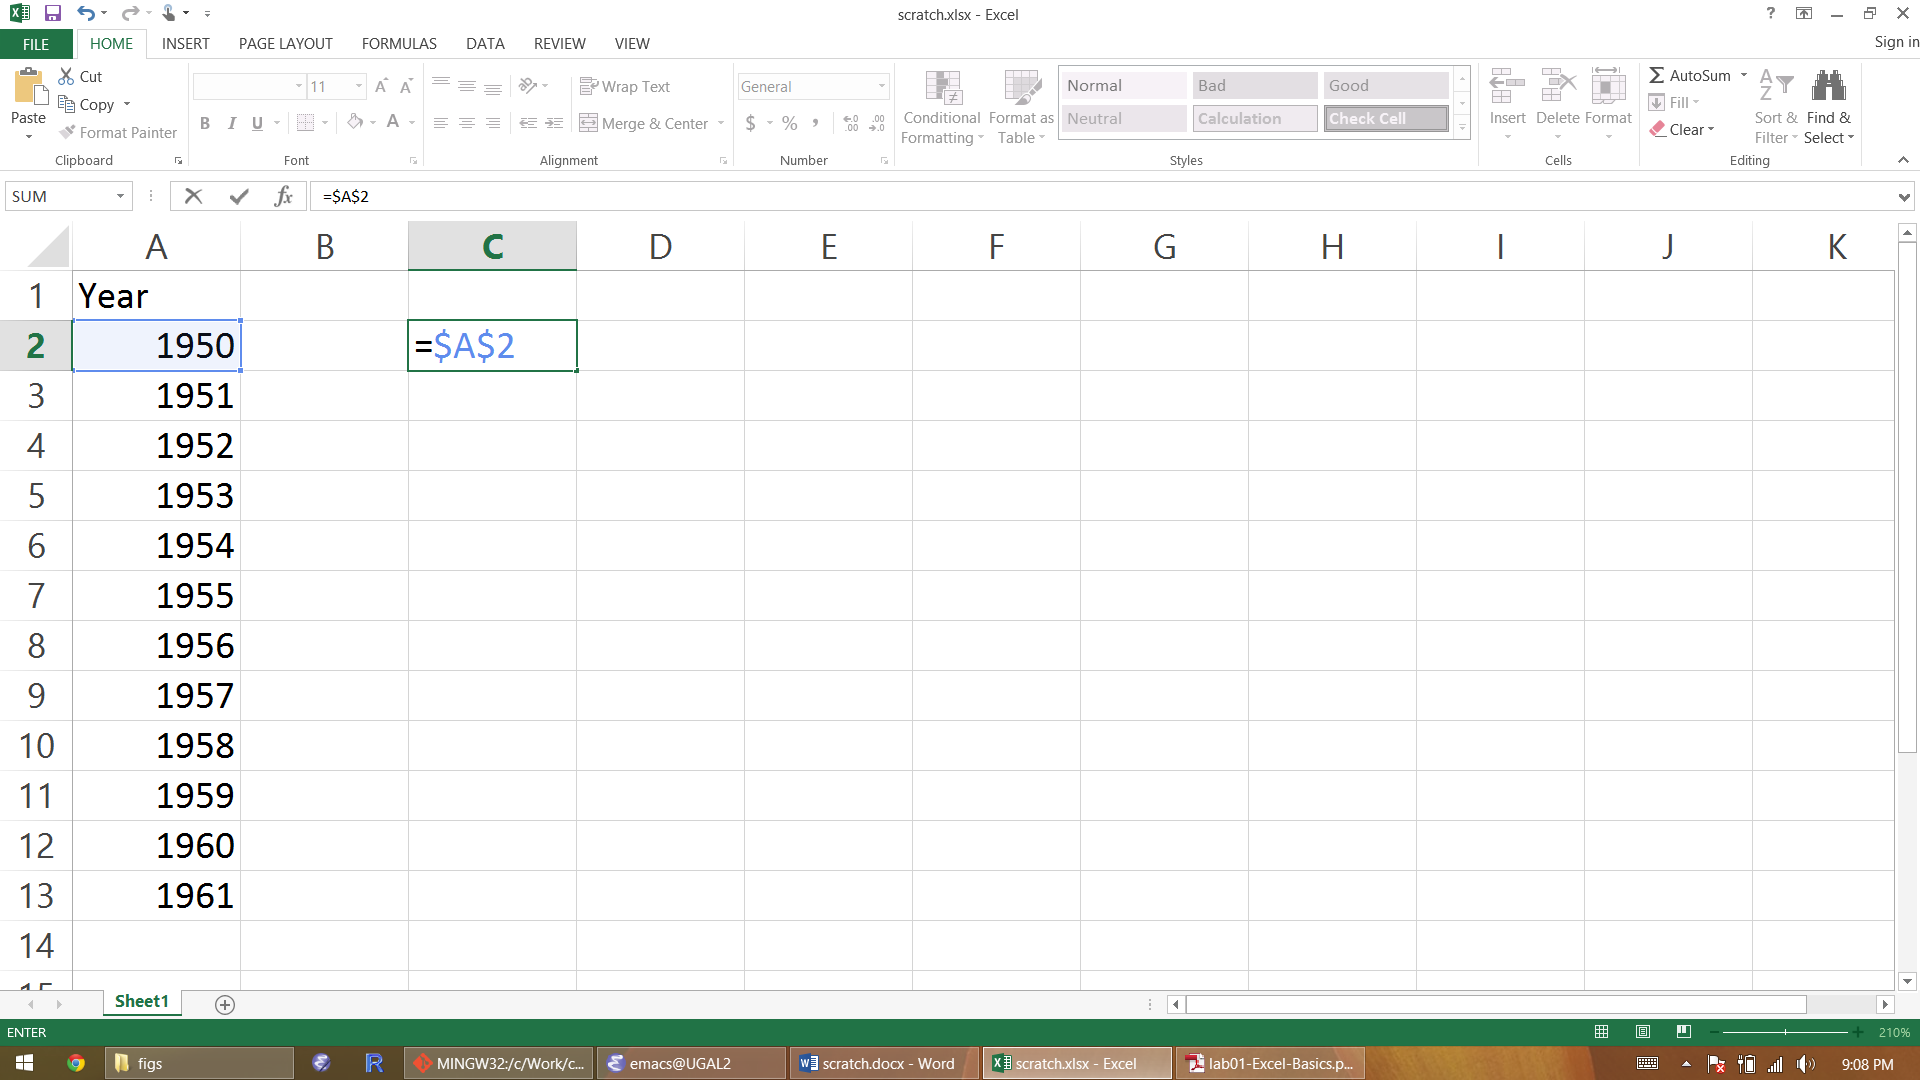
\includegraphics[width=\textwidth]{figs/absolute-ref}}}
  \only<2 | handout:0>{\fbox{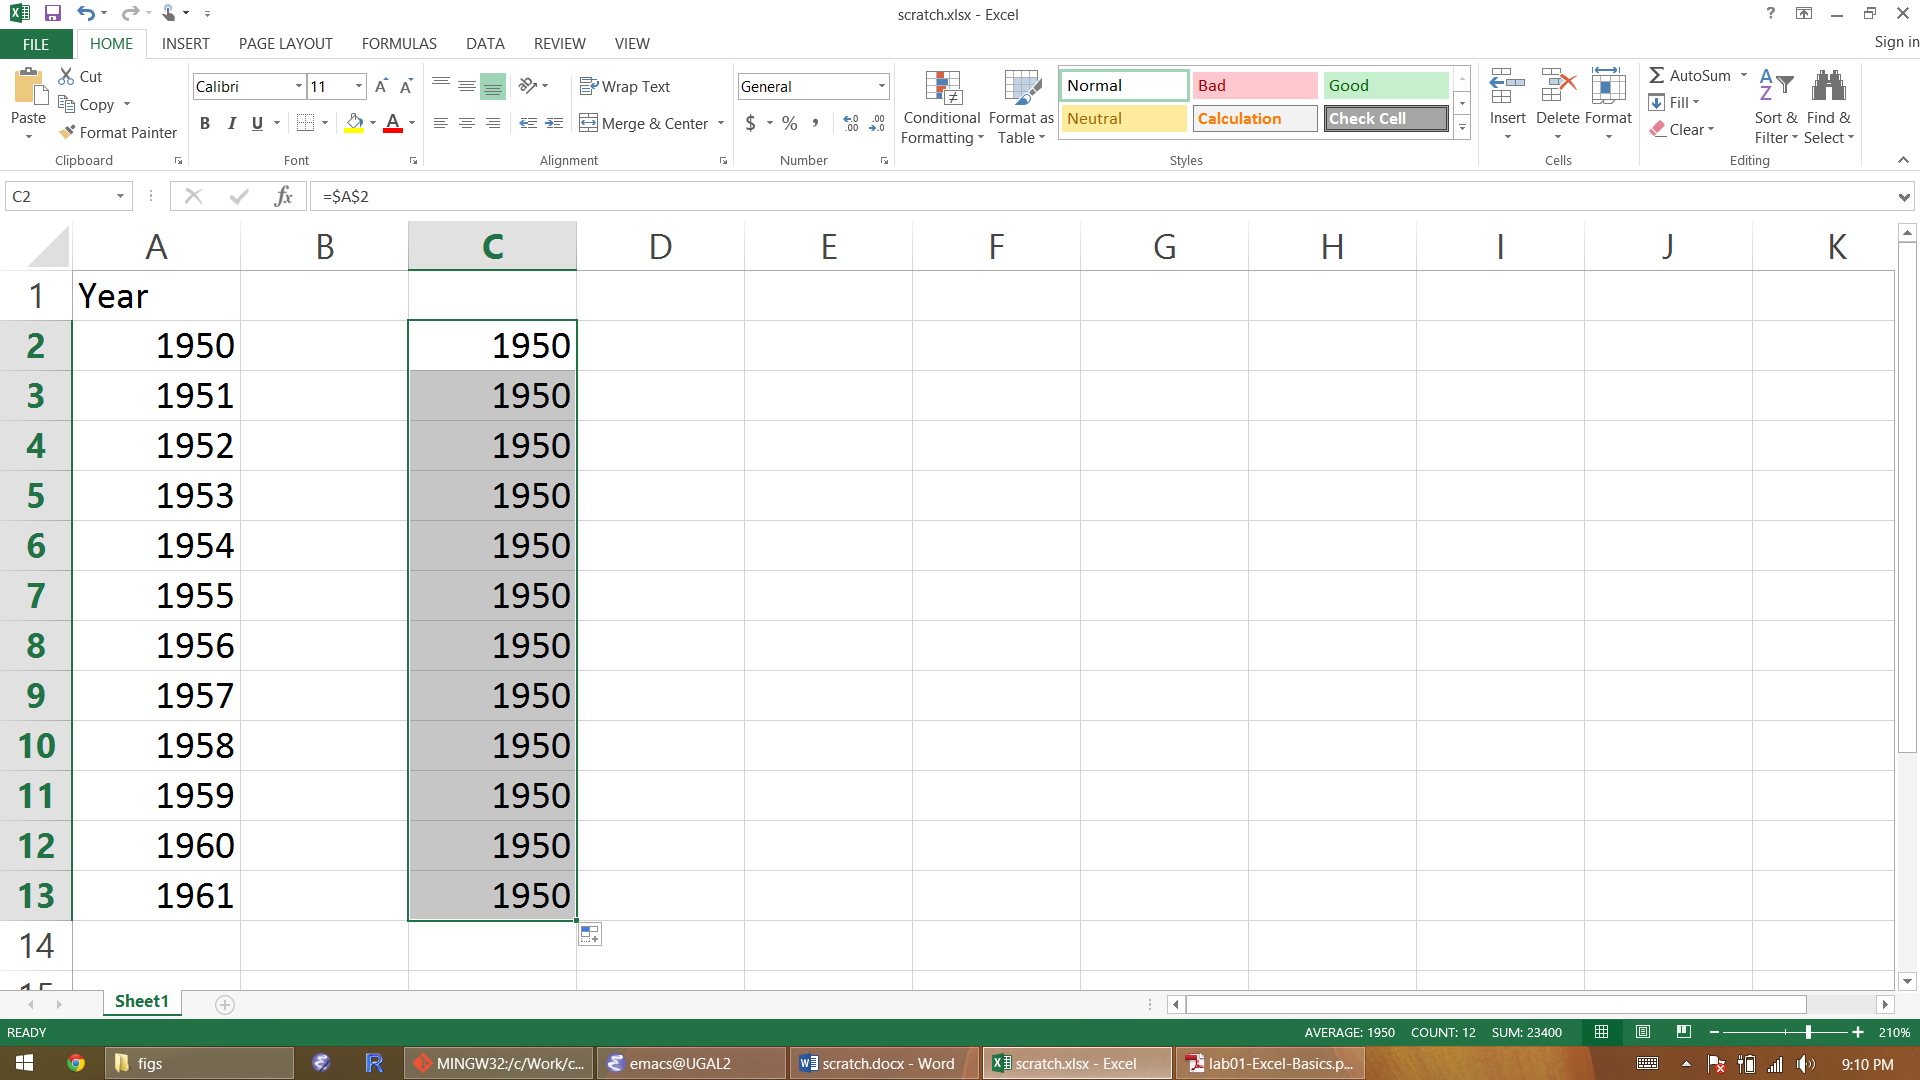
\includegraphics[width=\textwidth]{figs/absolute-ref2}}}
  \begin{center}
    Dollar sign ``locks'' a reference so that auto-fill won't change it
  \end{center}
\end{frame}


\begin{frame}
  \frametitle{Partial Cell References}
  \fbox{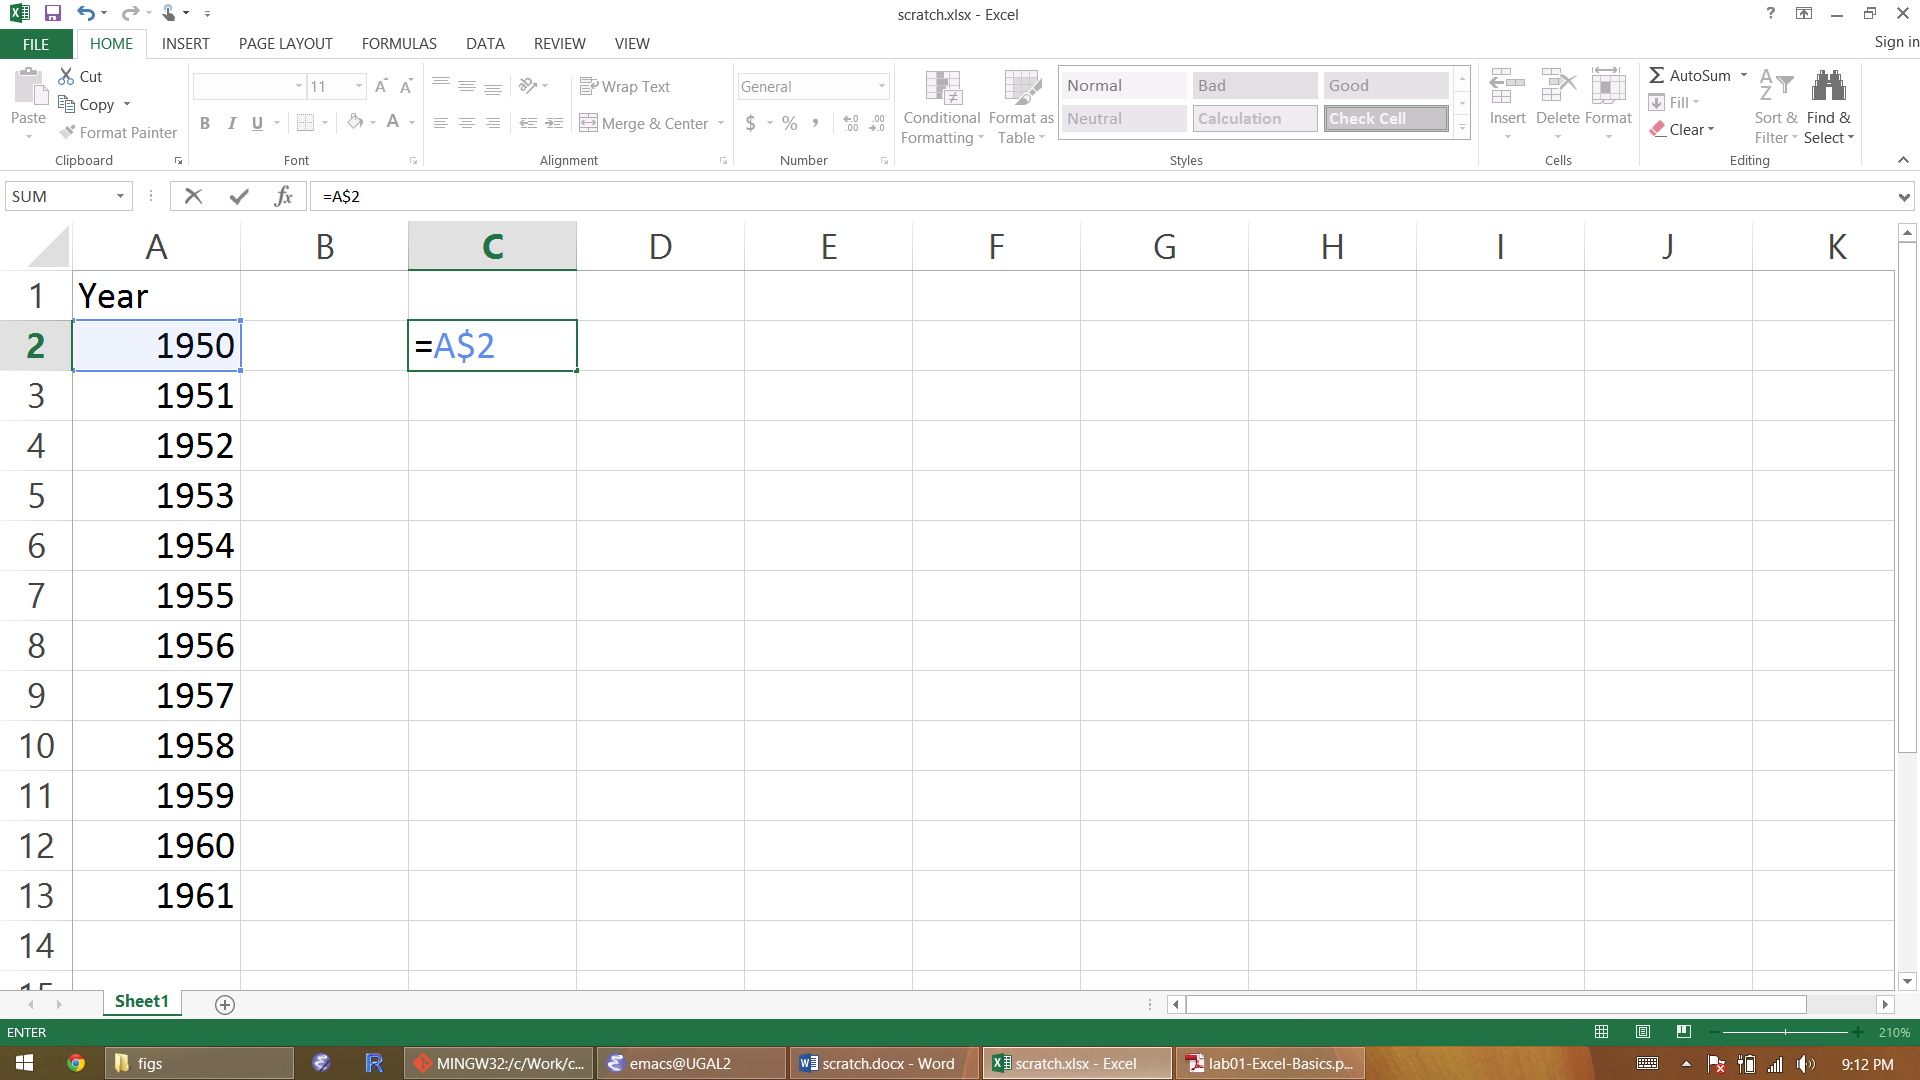
\includegraphics[width=\textwidth]{figs/partial-ref}}
\end{frame}


\section{Equations}



\begin{frame}
  \frametitle{Equations}
    \only<1>{\fbox{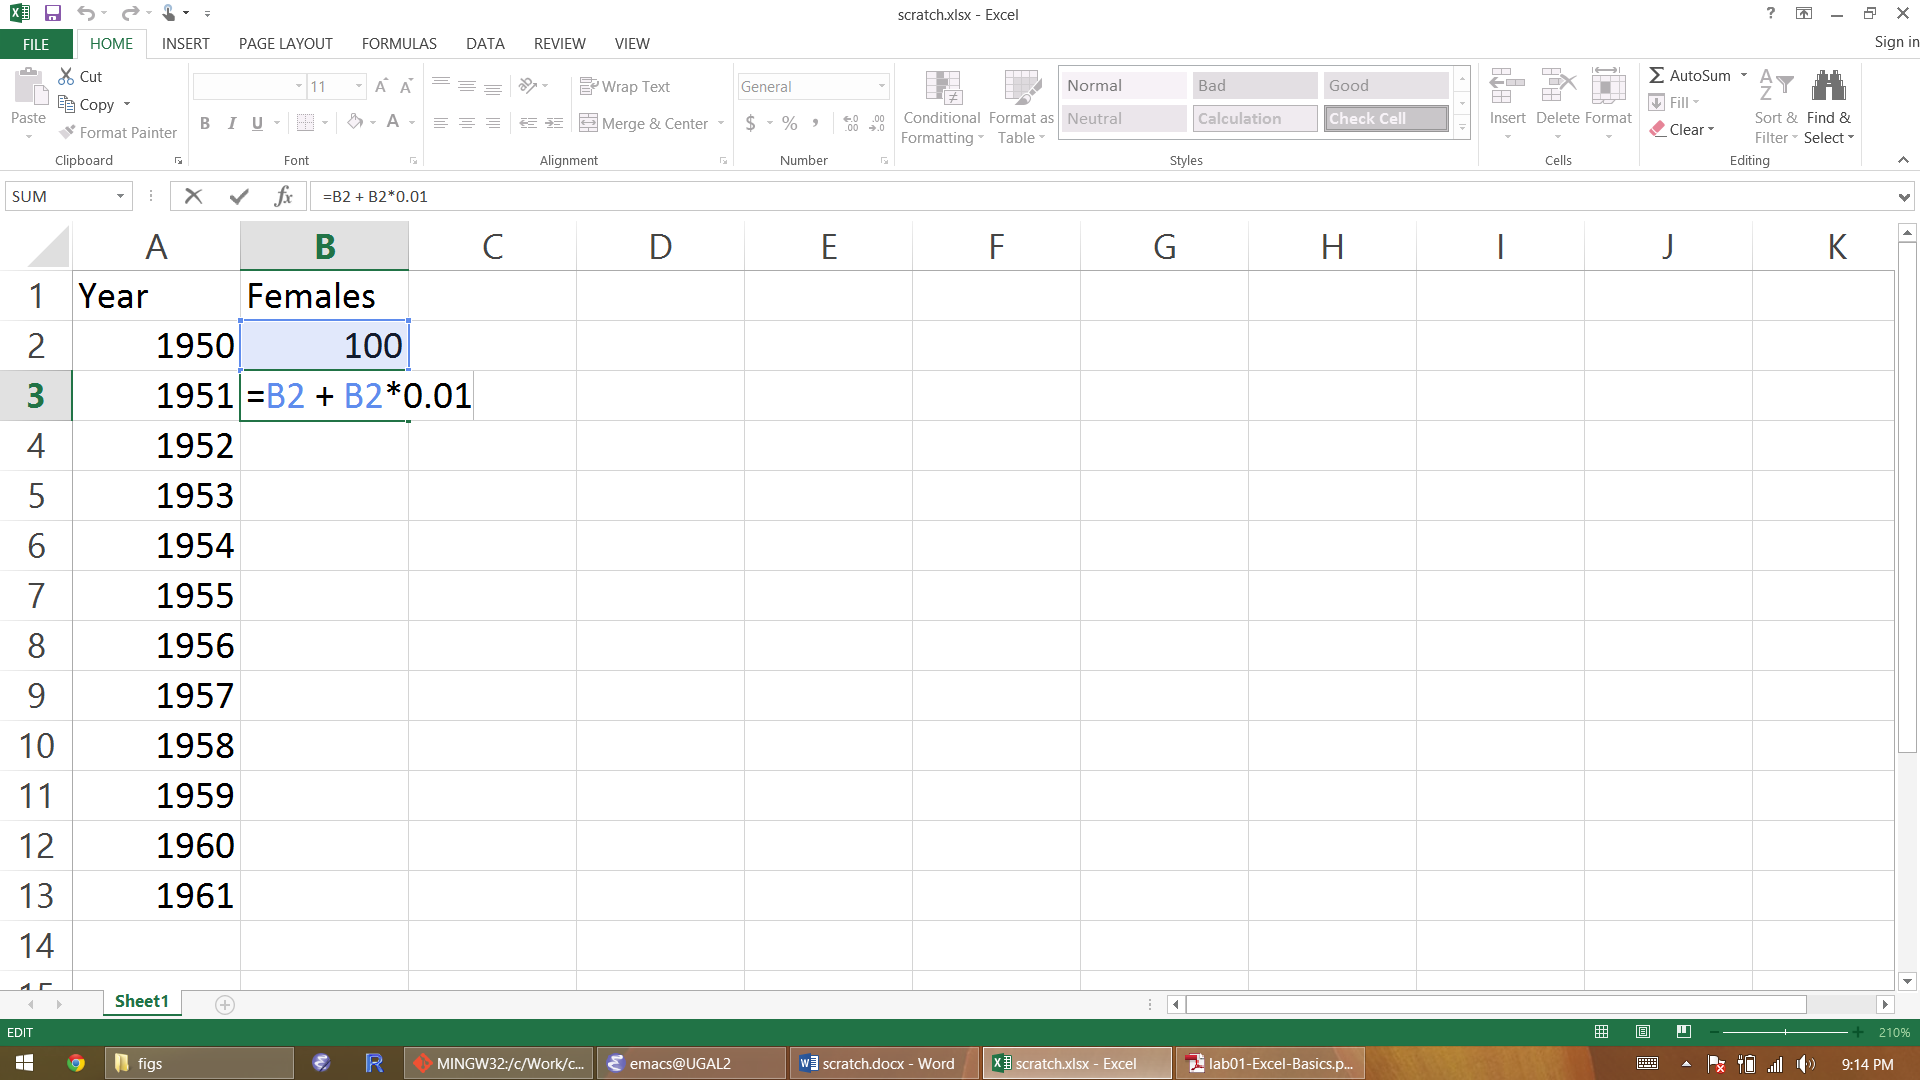
\includegraphics[width=\textwidth]{figs/equation}}}
    \only<2 | handout:0>{\fbox{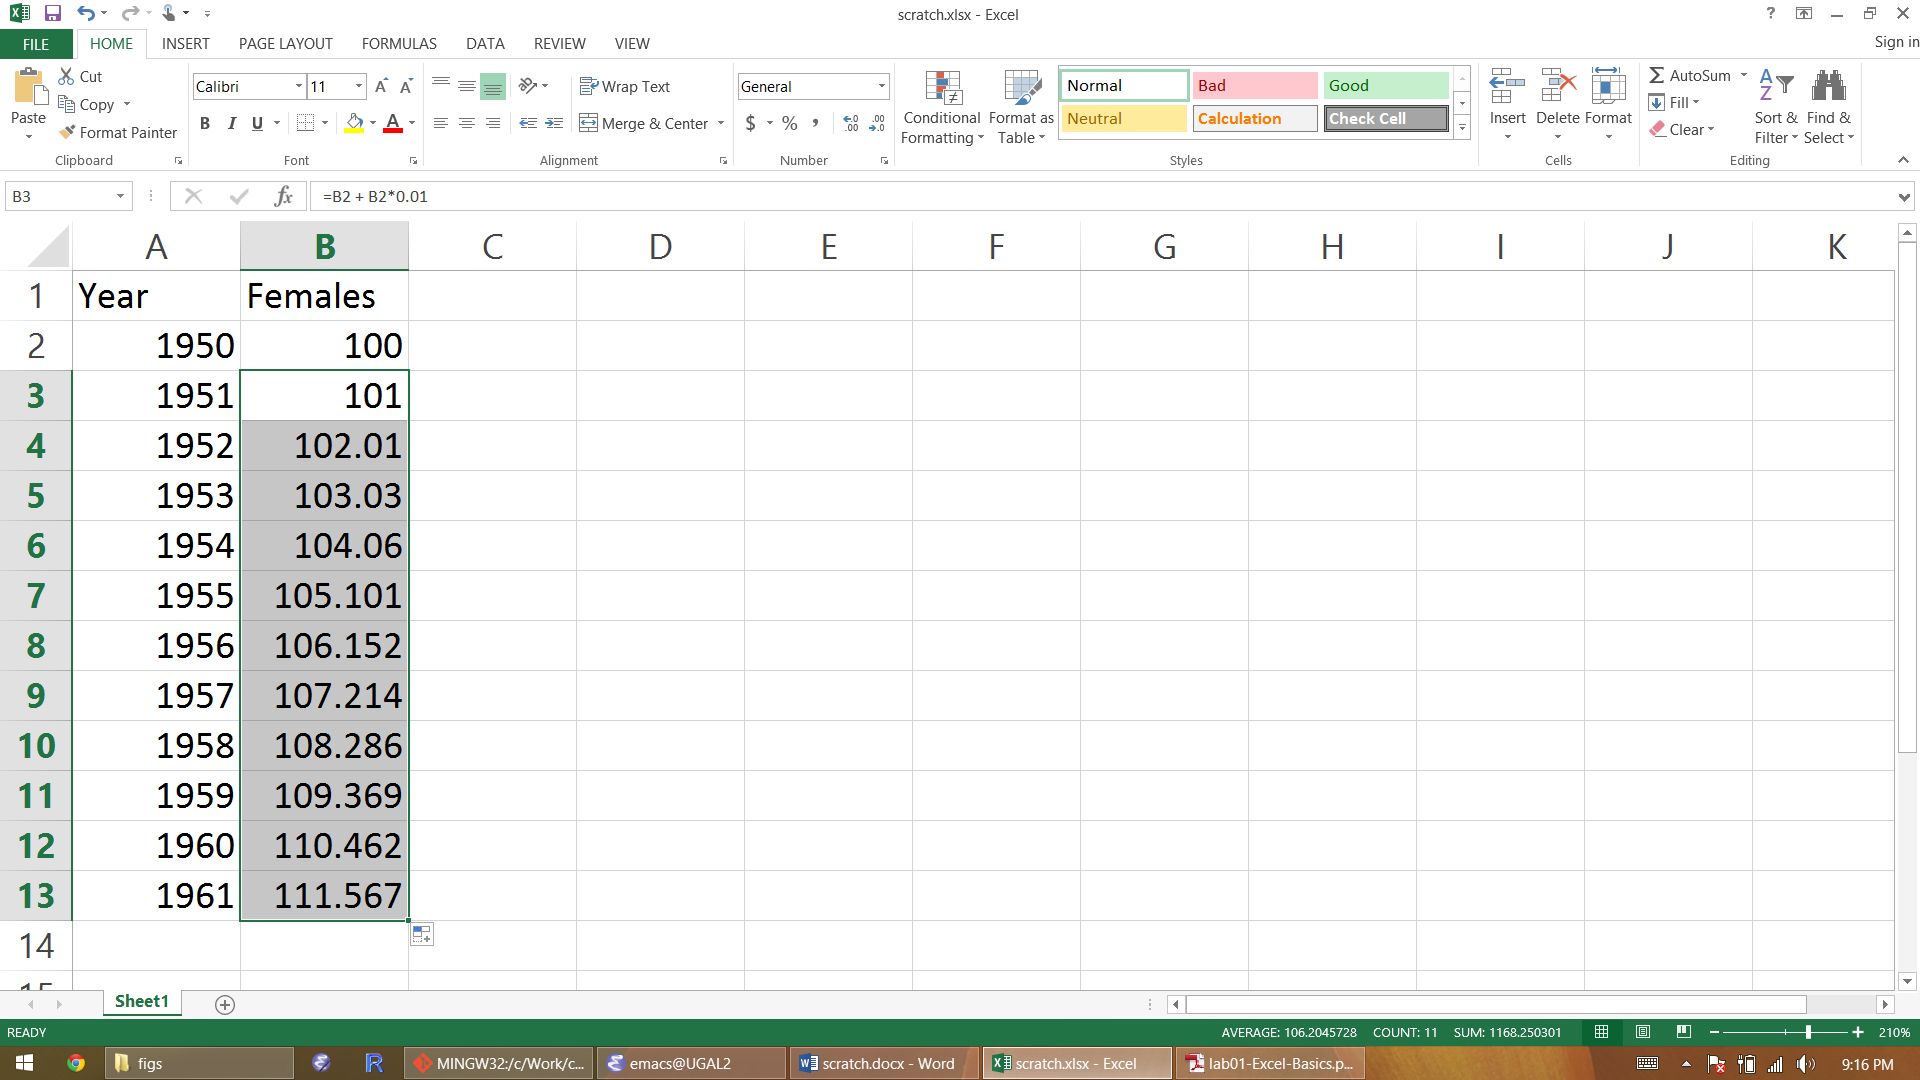
\includegraphics[width=\textwidth]{figs/equation2}}}
\end{frame}



\begin{frame}
  \frametitle{Equations}
    \only<1>{\fbox{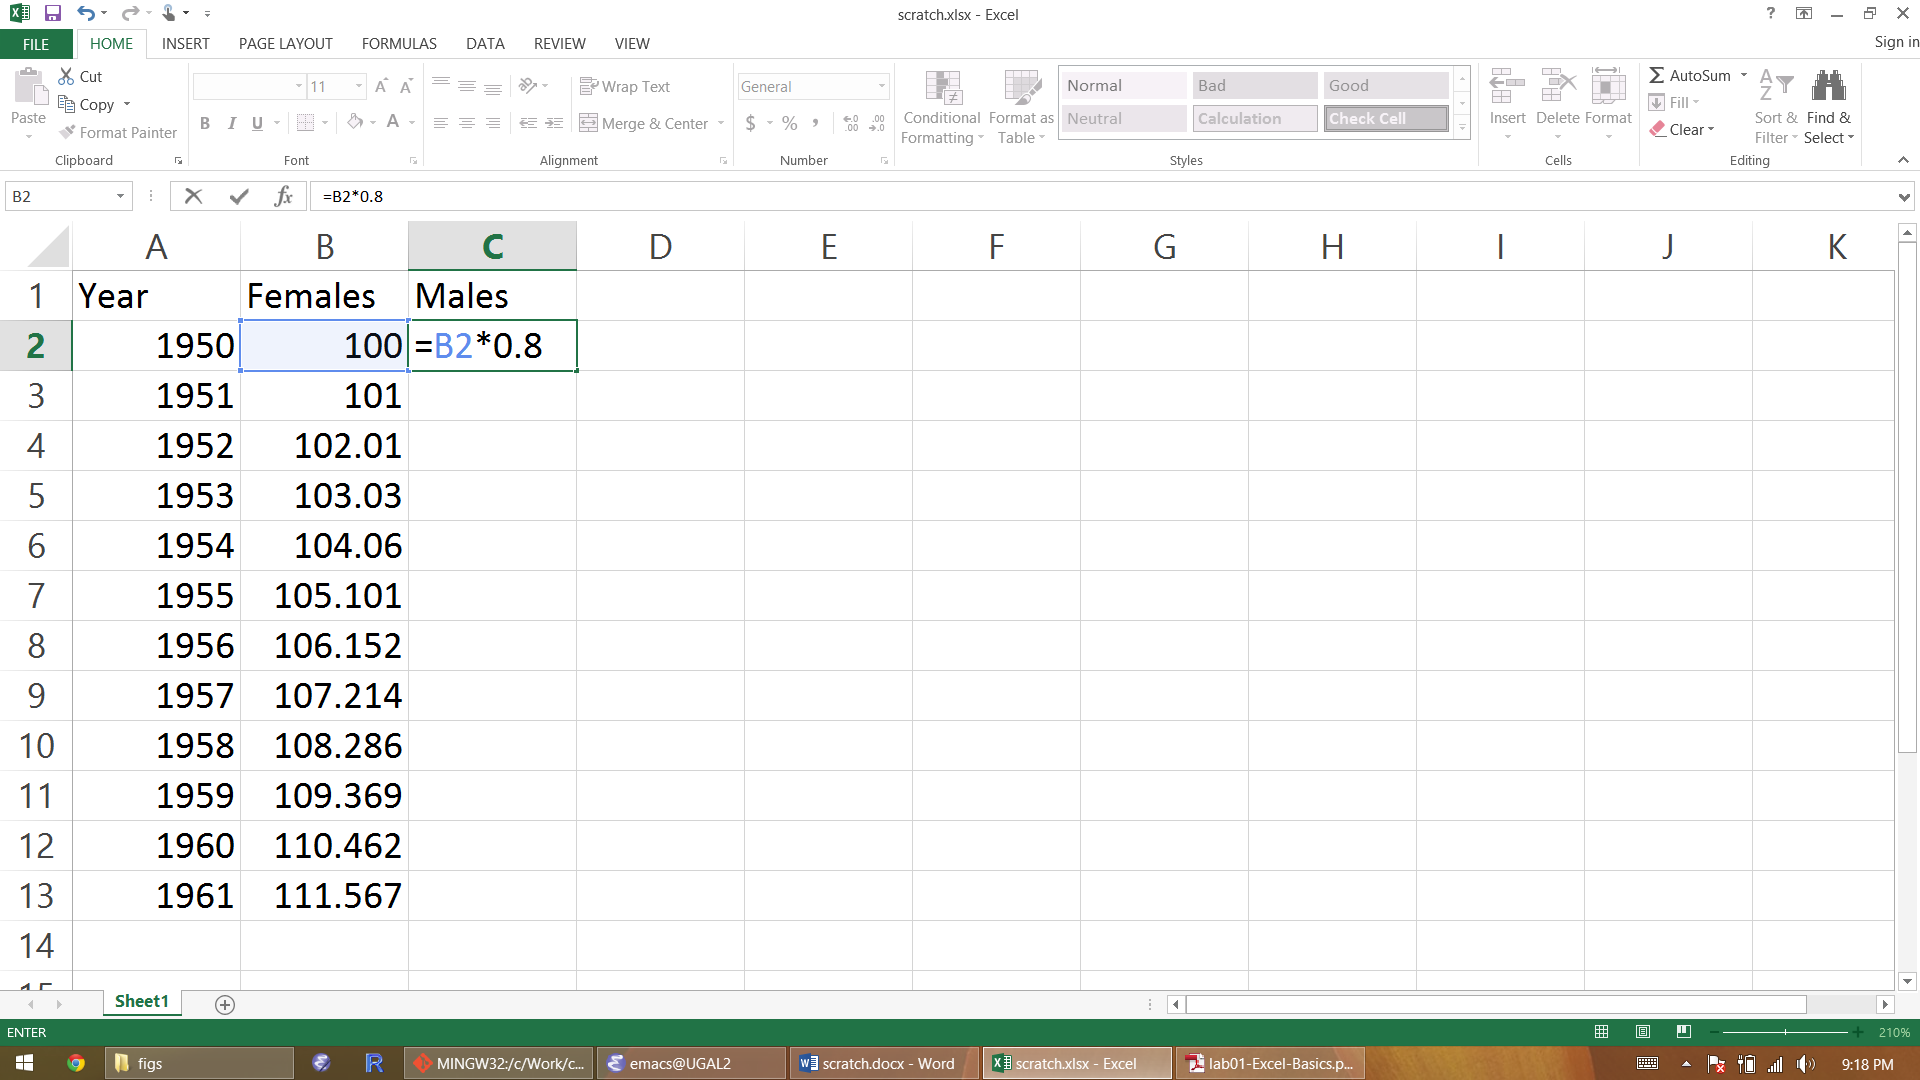
\includegraphics[width=\textwidth]{figs/equation3}}}
    \only<2 | handout:0>{\fbox{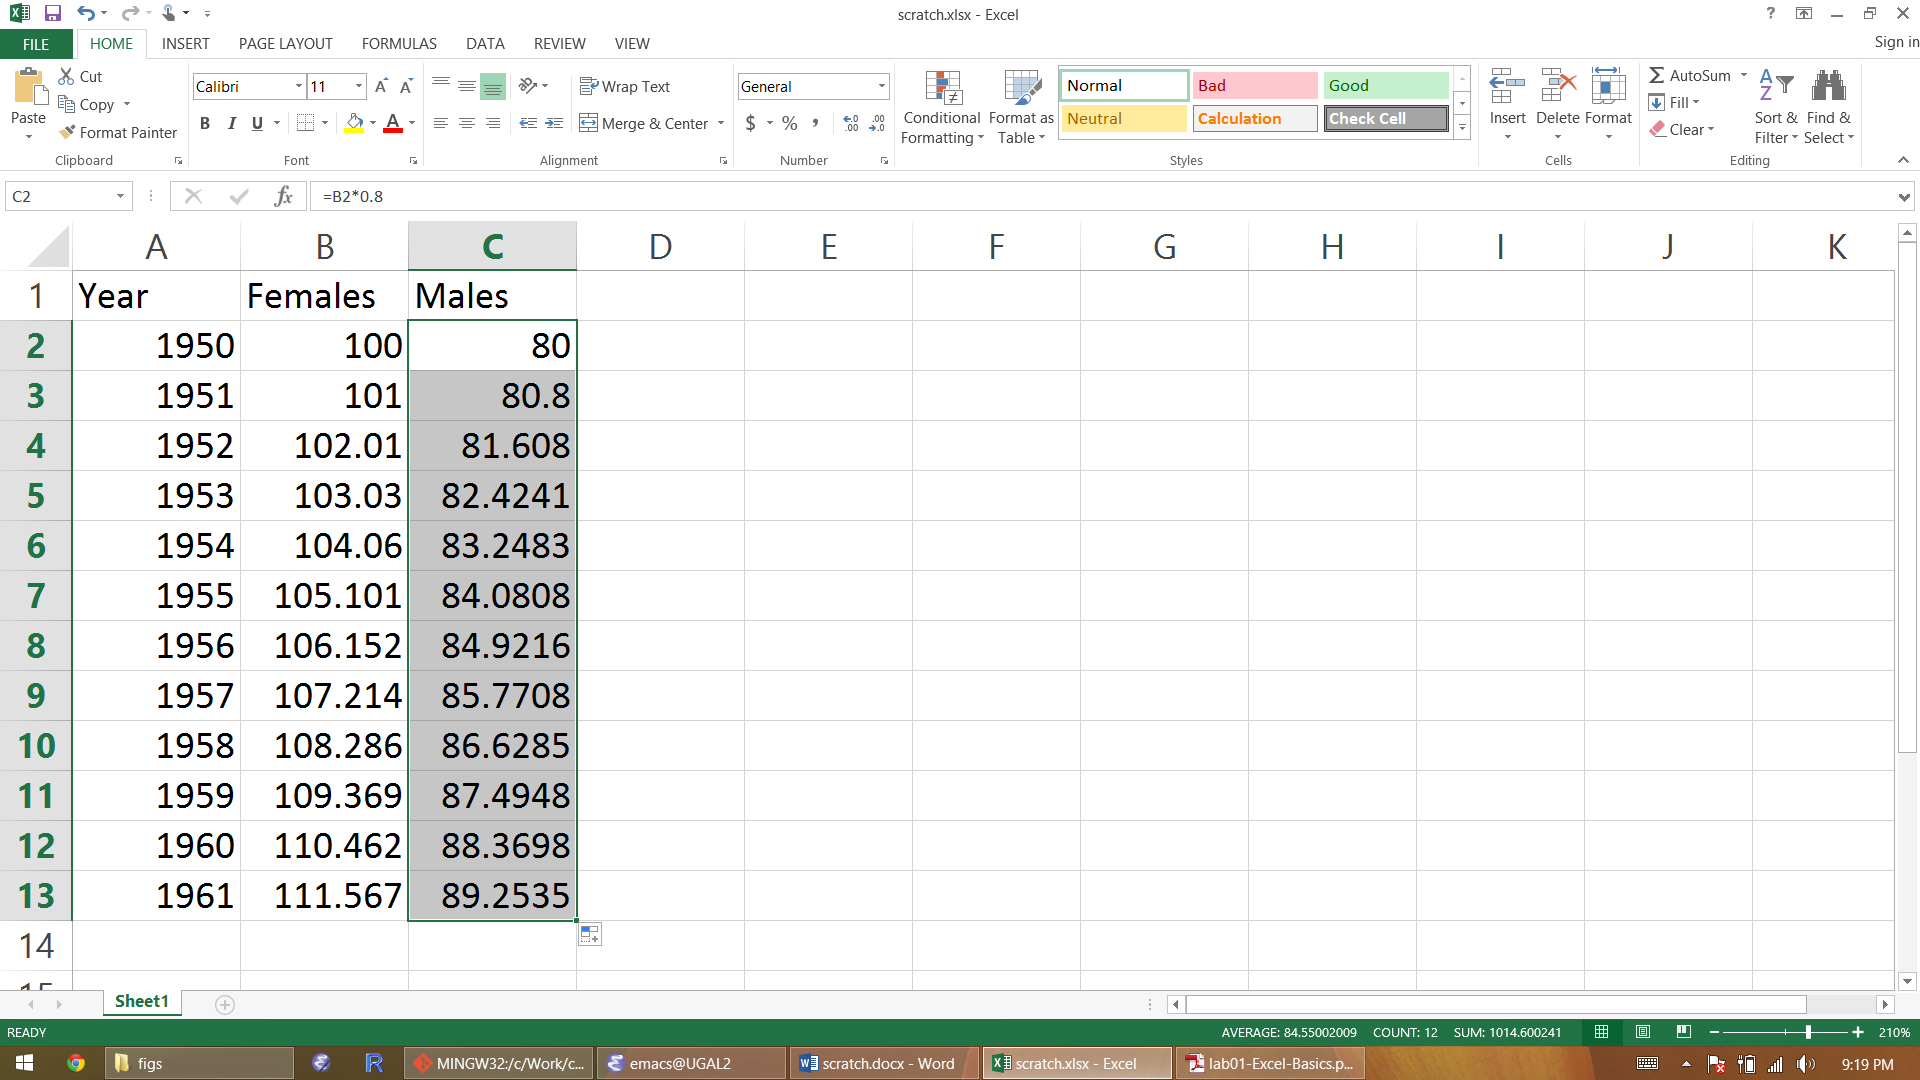
\includegraphics[width=\textwidth]{figs/equation4}}}
\end{frame}



\begin{frame}
  \frametitle{Formulas}
  \fbox{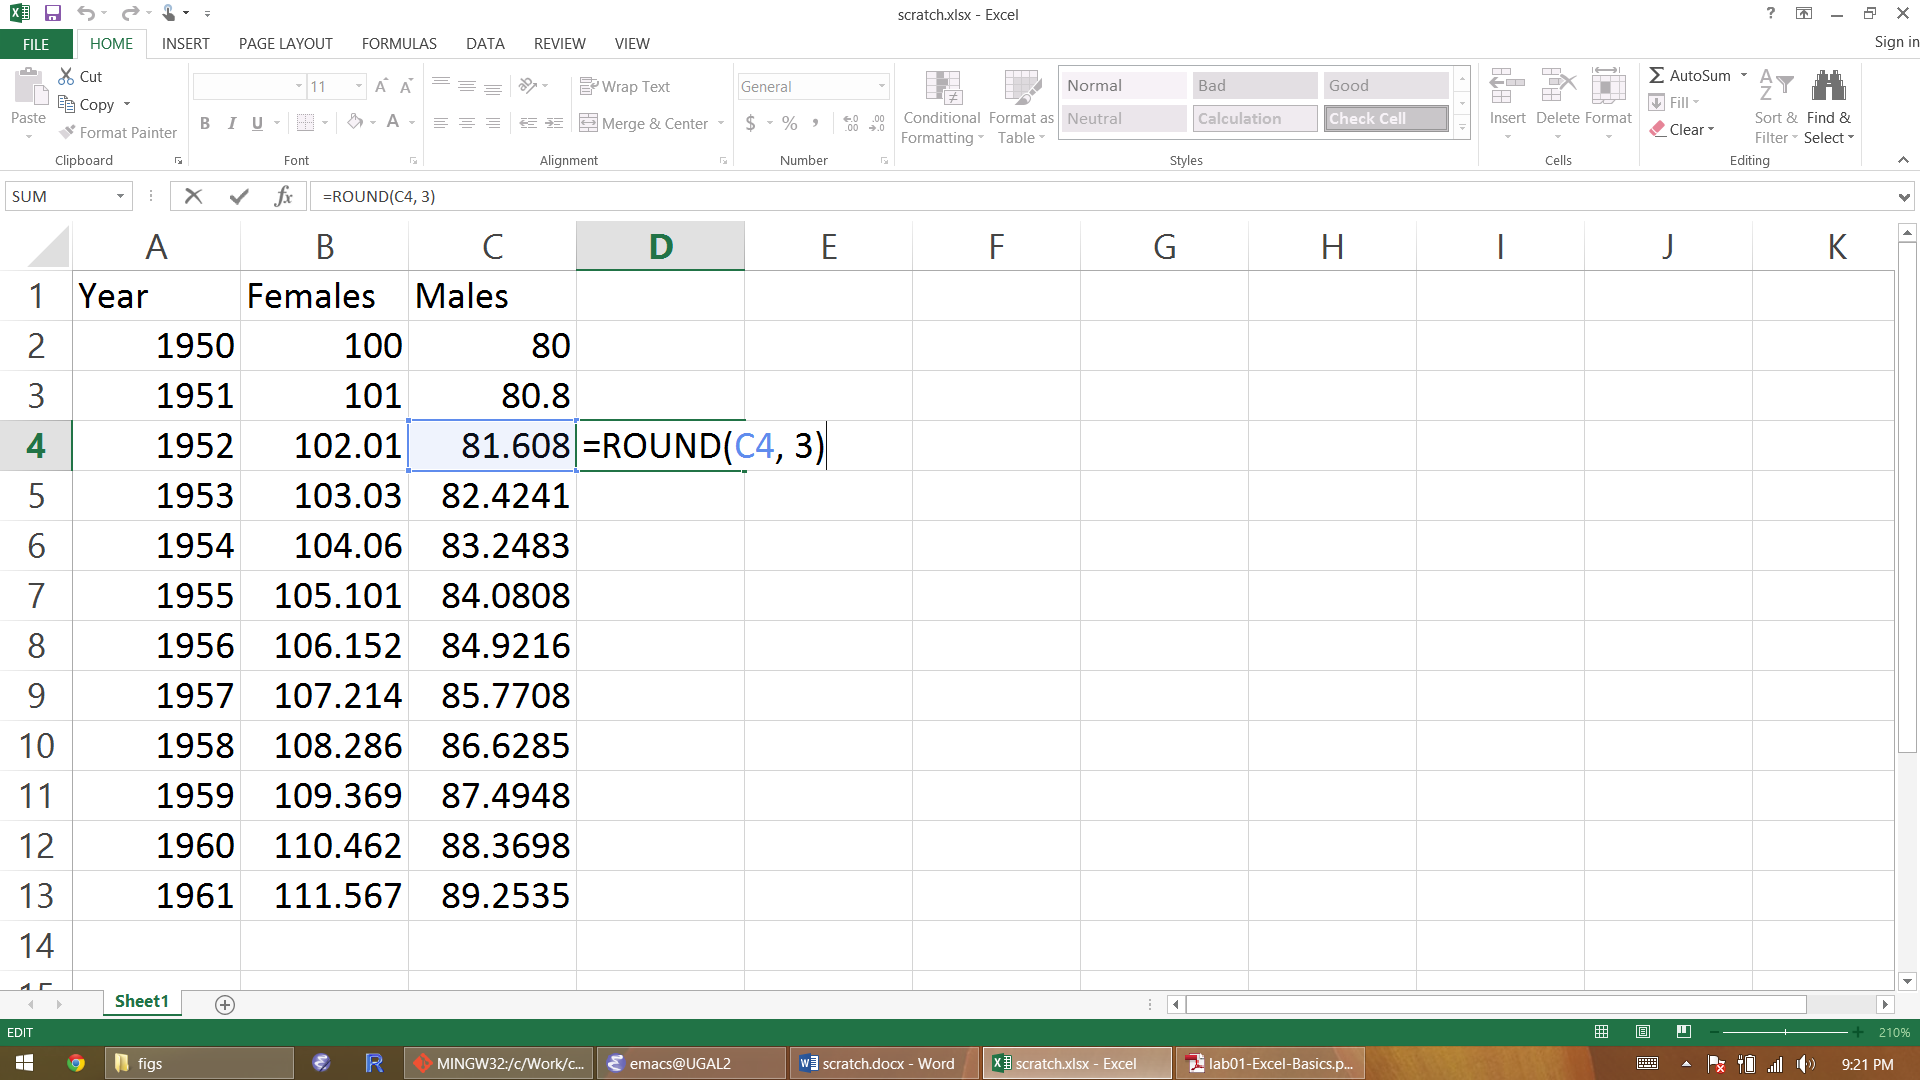
\includegraphics[width=\textwidth]{figs/formula}}
\end{frame}


\section{Graphics}



\begin{frame}
  \frametitle{Graphics}
    \fbox{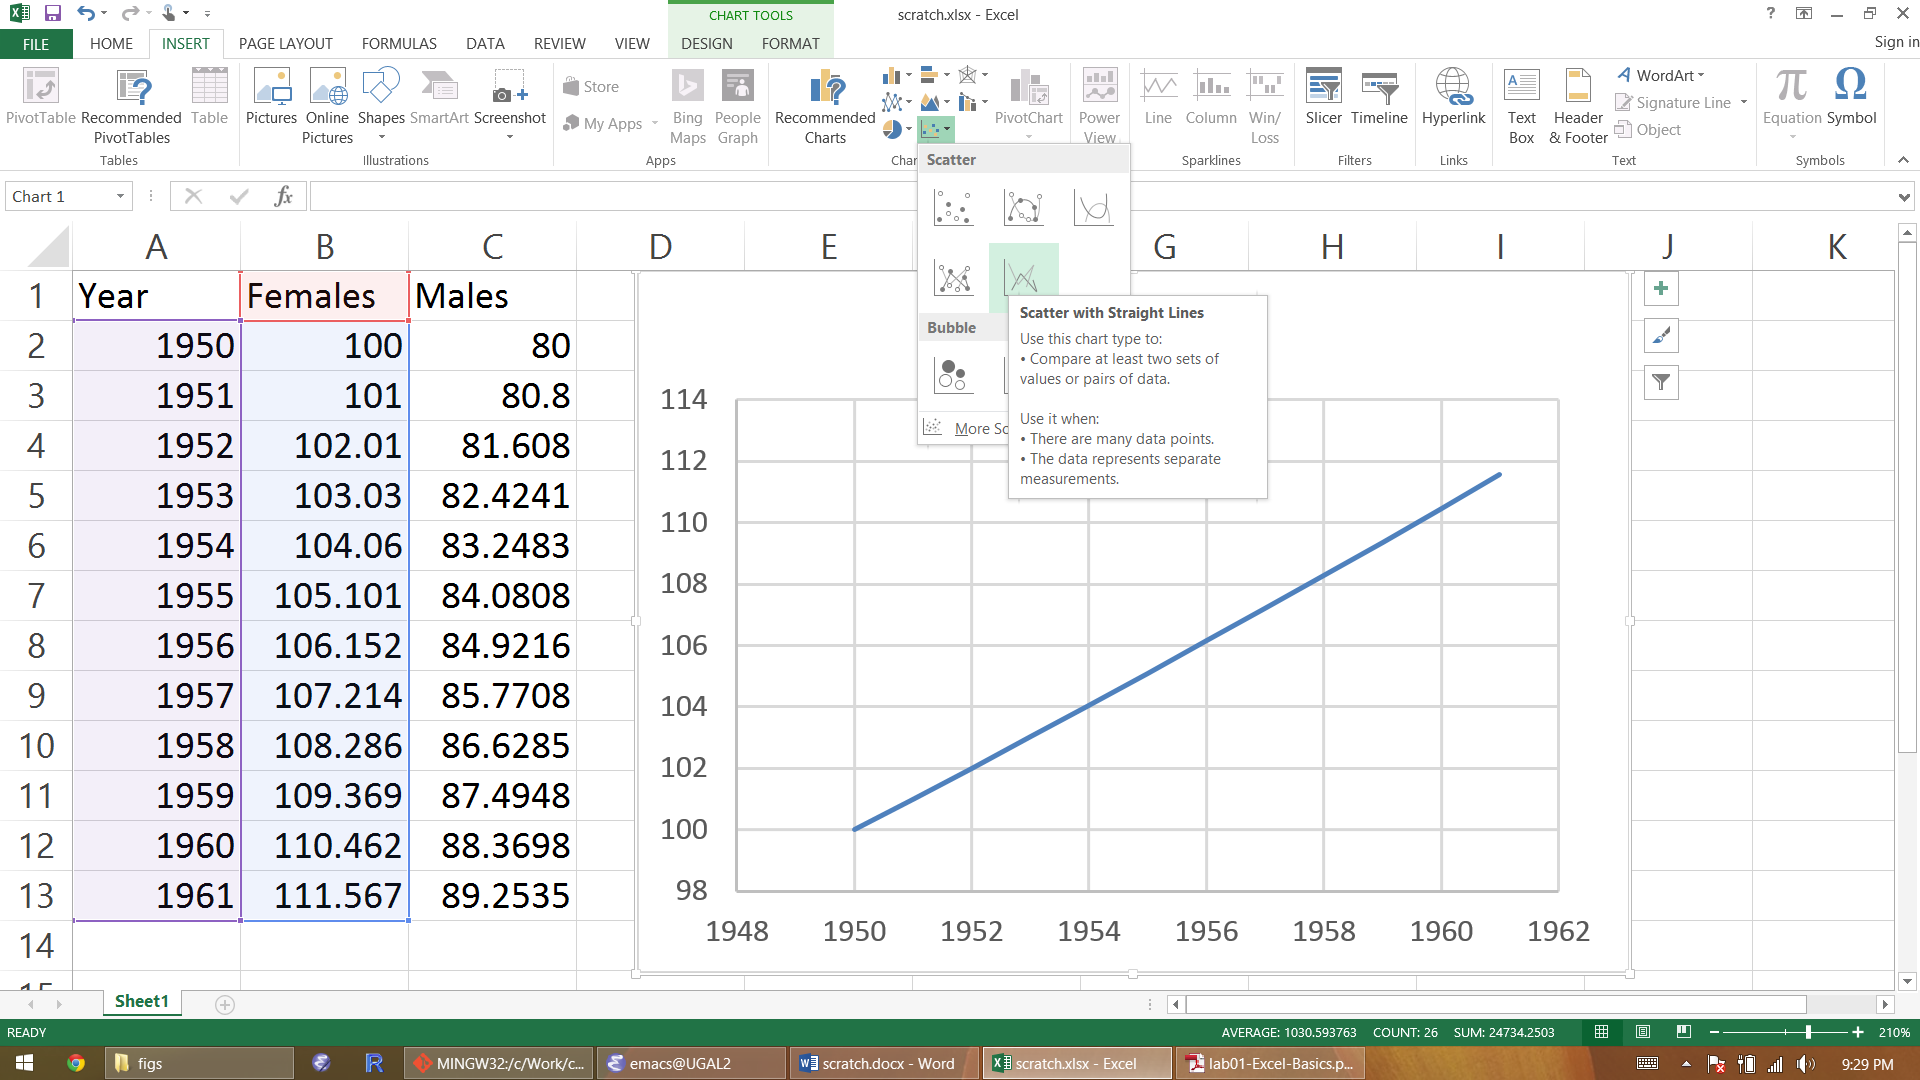
\includegraphics[width=\textwidth]{figs/scatterlines}}
\end{frame}


\begin{frame}
  \frametitle{Graphics}
  \only<1>{\fbox{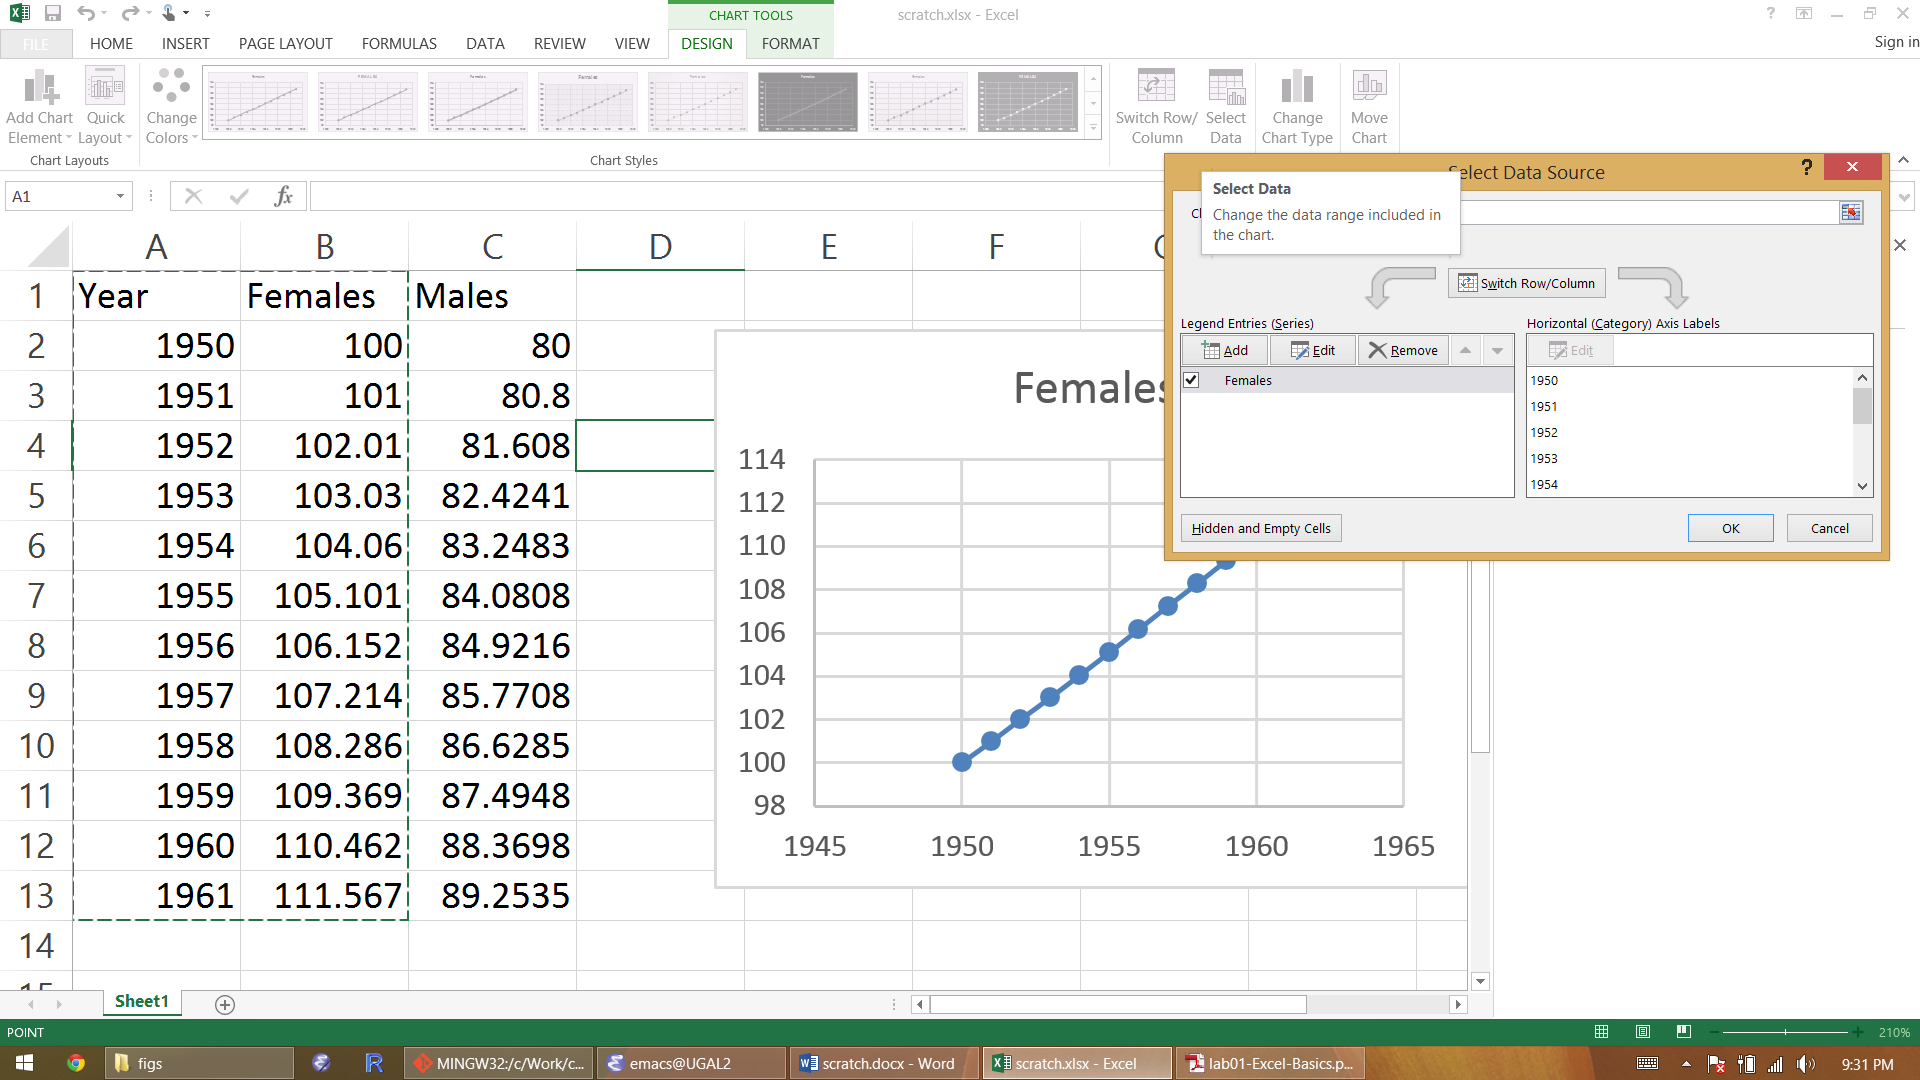
\includegraphics[width=\textwidth]{figs/scatterlines2}}}
  \only<2 | handout:0>{\fbox{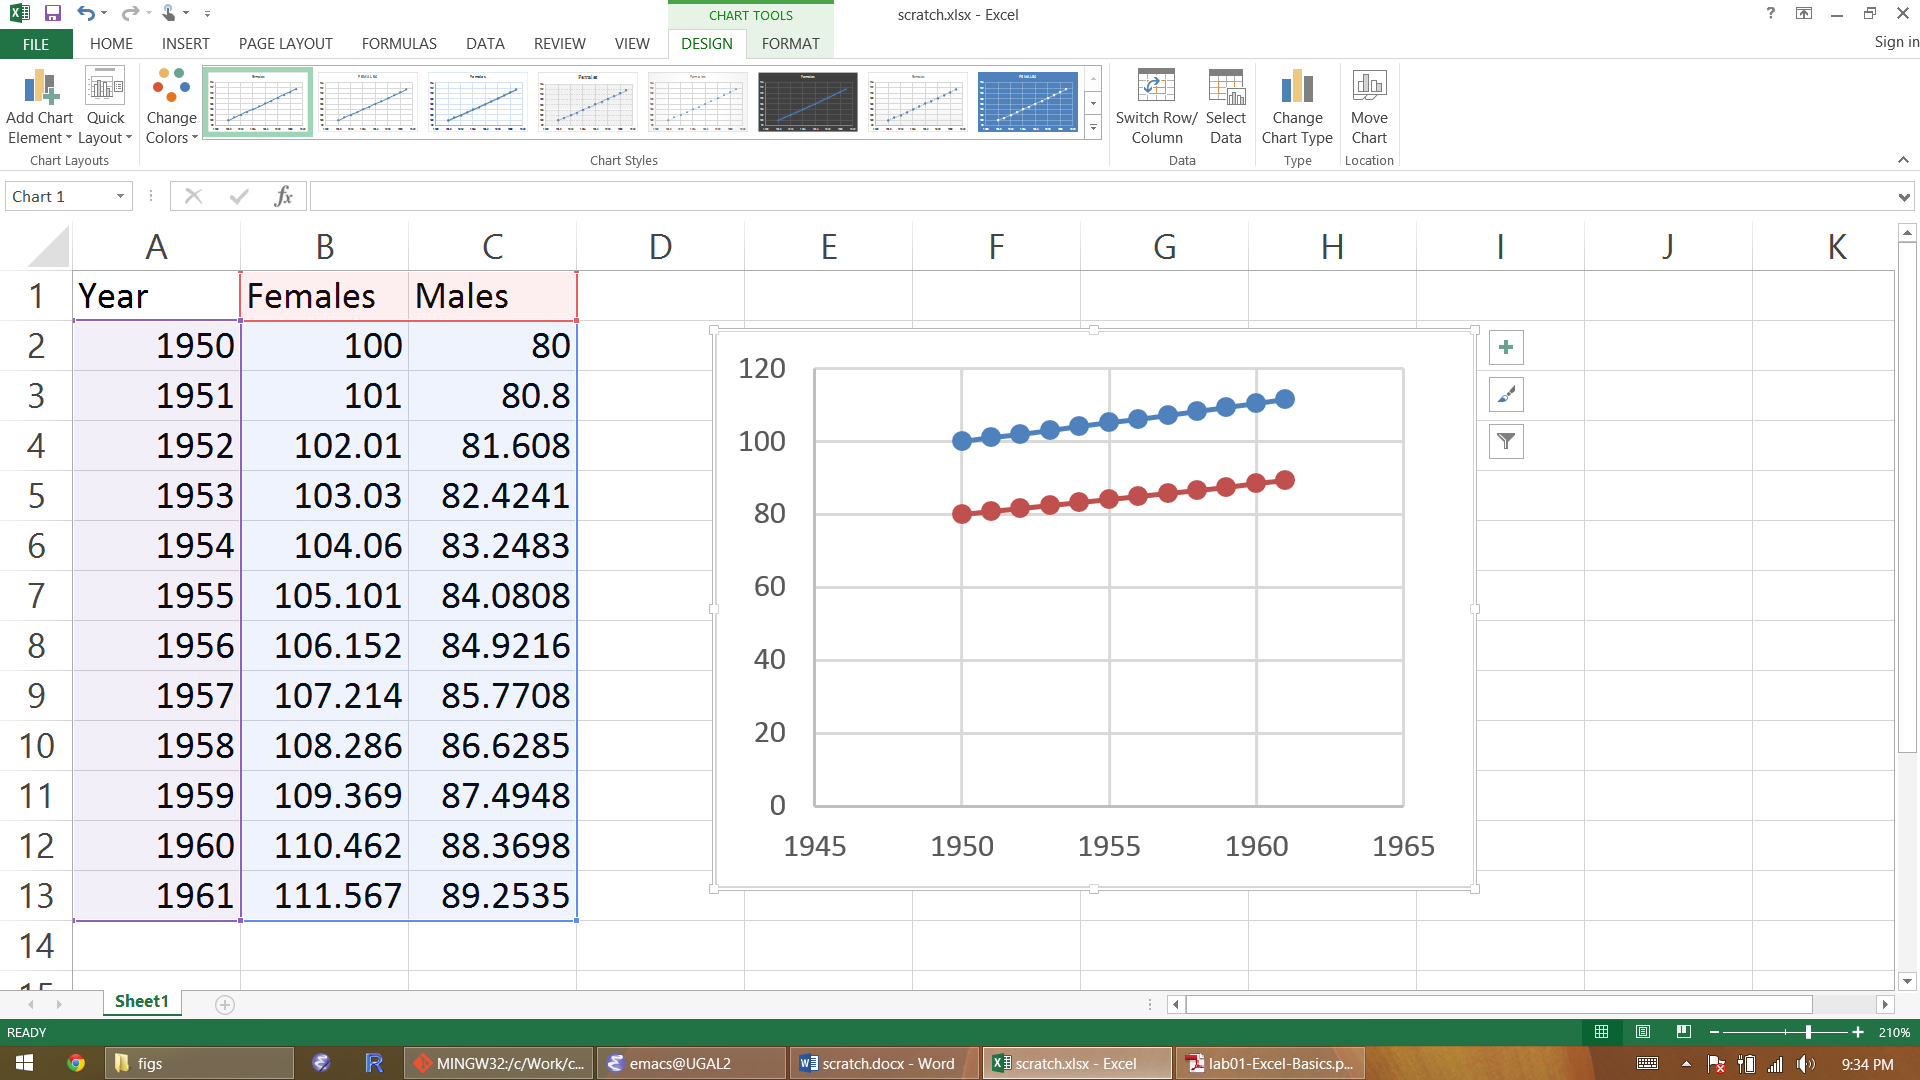
\includegraphics[width=\textwidth]{figs/scatterlines3}}}
  \begin{center}
    Add a line for males
  \end{center}
\end{frame}





\begin{frame}
  \frametitle{Customize}
    \only<1>{\fbox{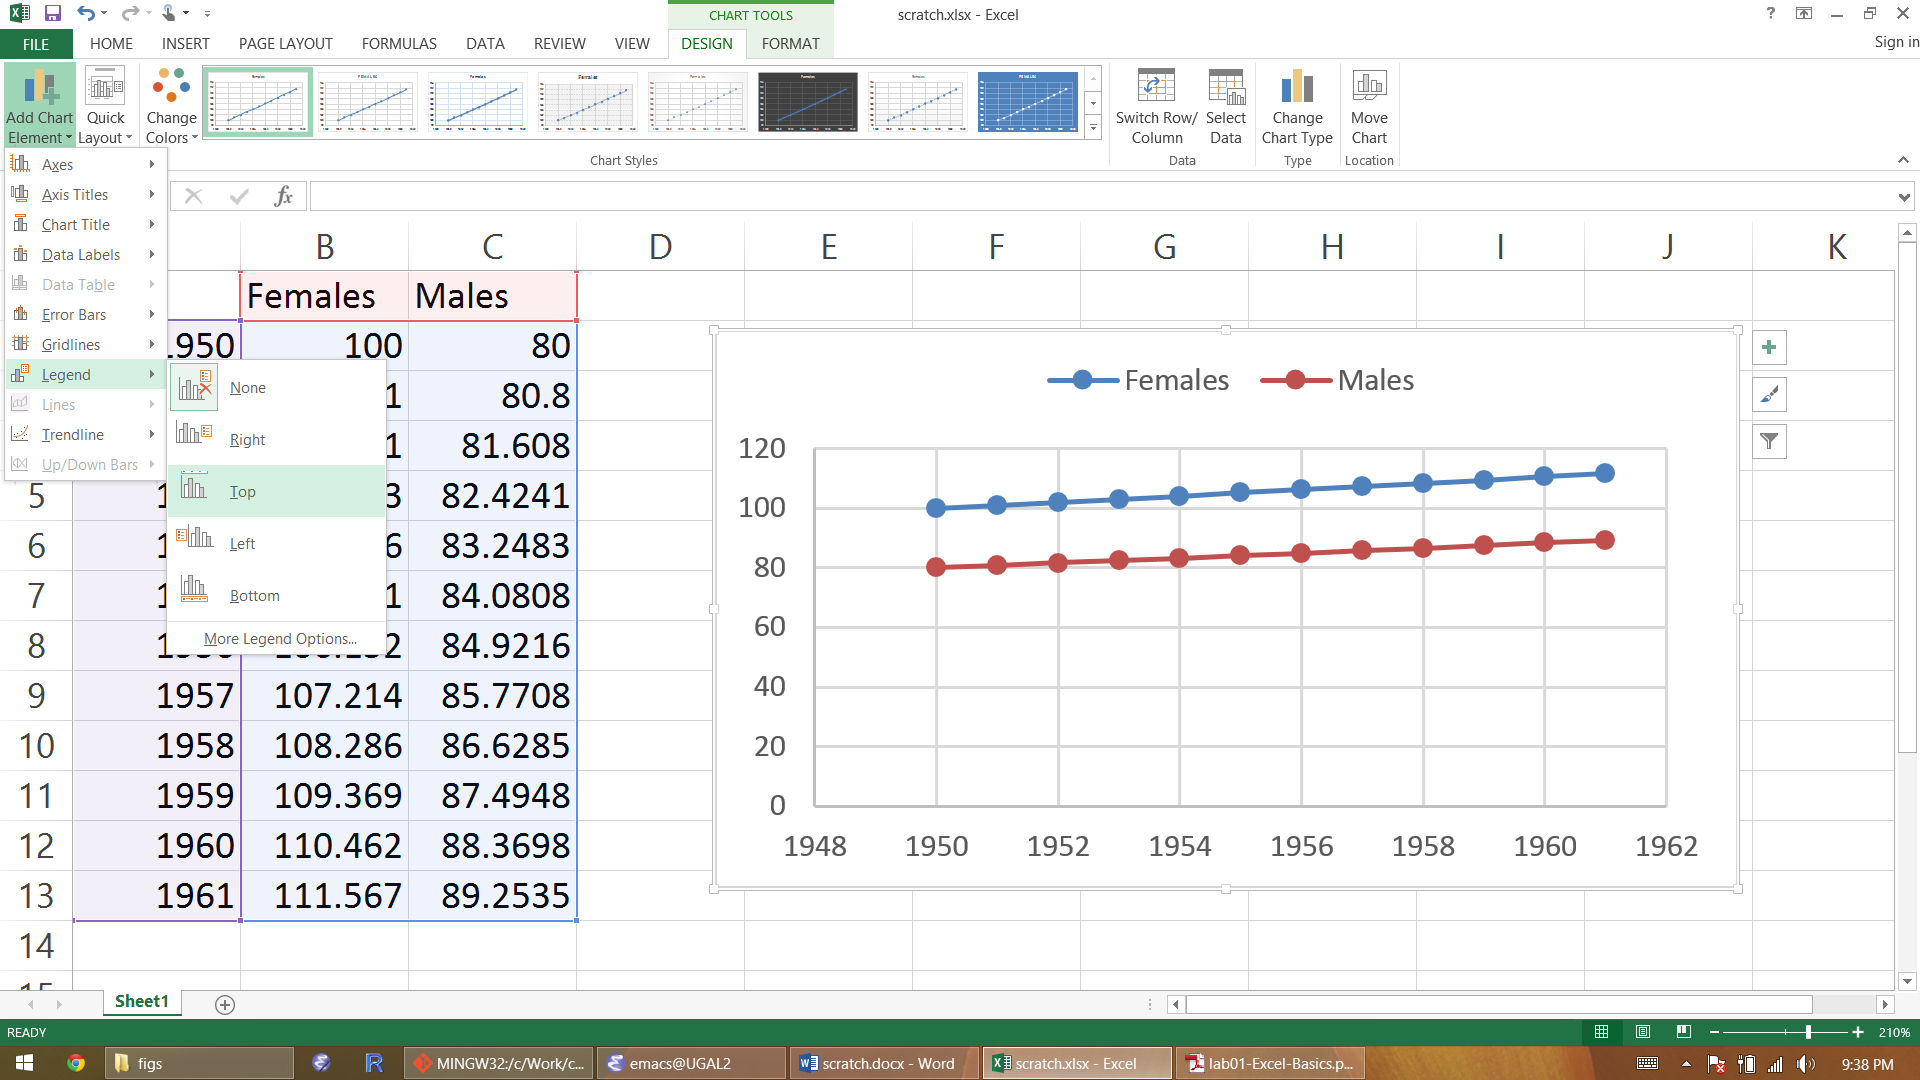
\includegraphics[width=\textwidth]{figs/customize}}}
    \begin{center}
      Add legend
    \end{center}
\end{frame}



\begin{frame}
  \frametitle{Customize}
    \fbox{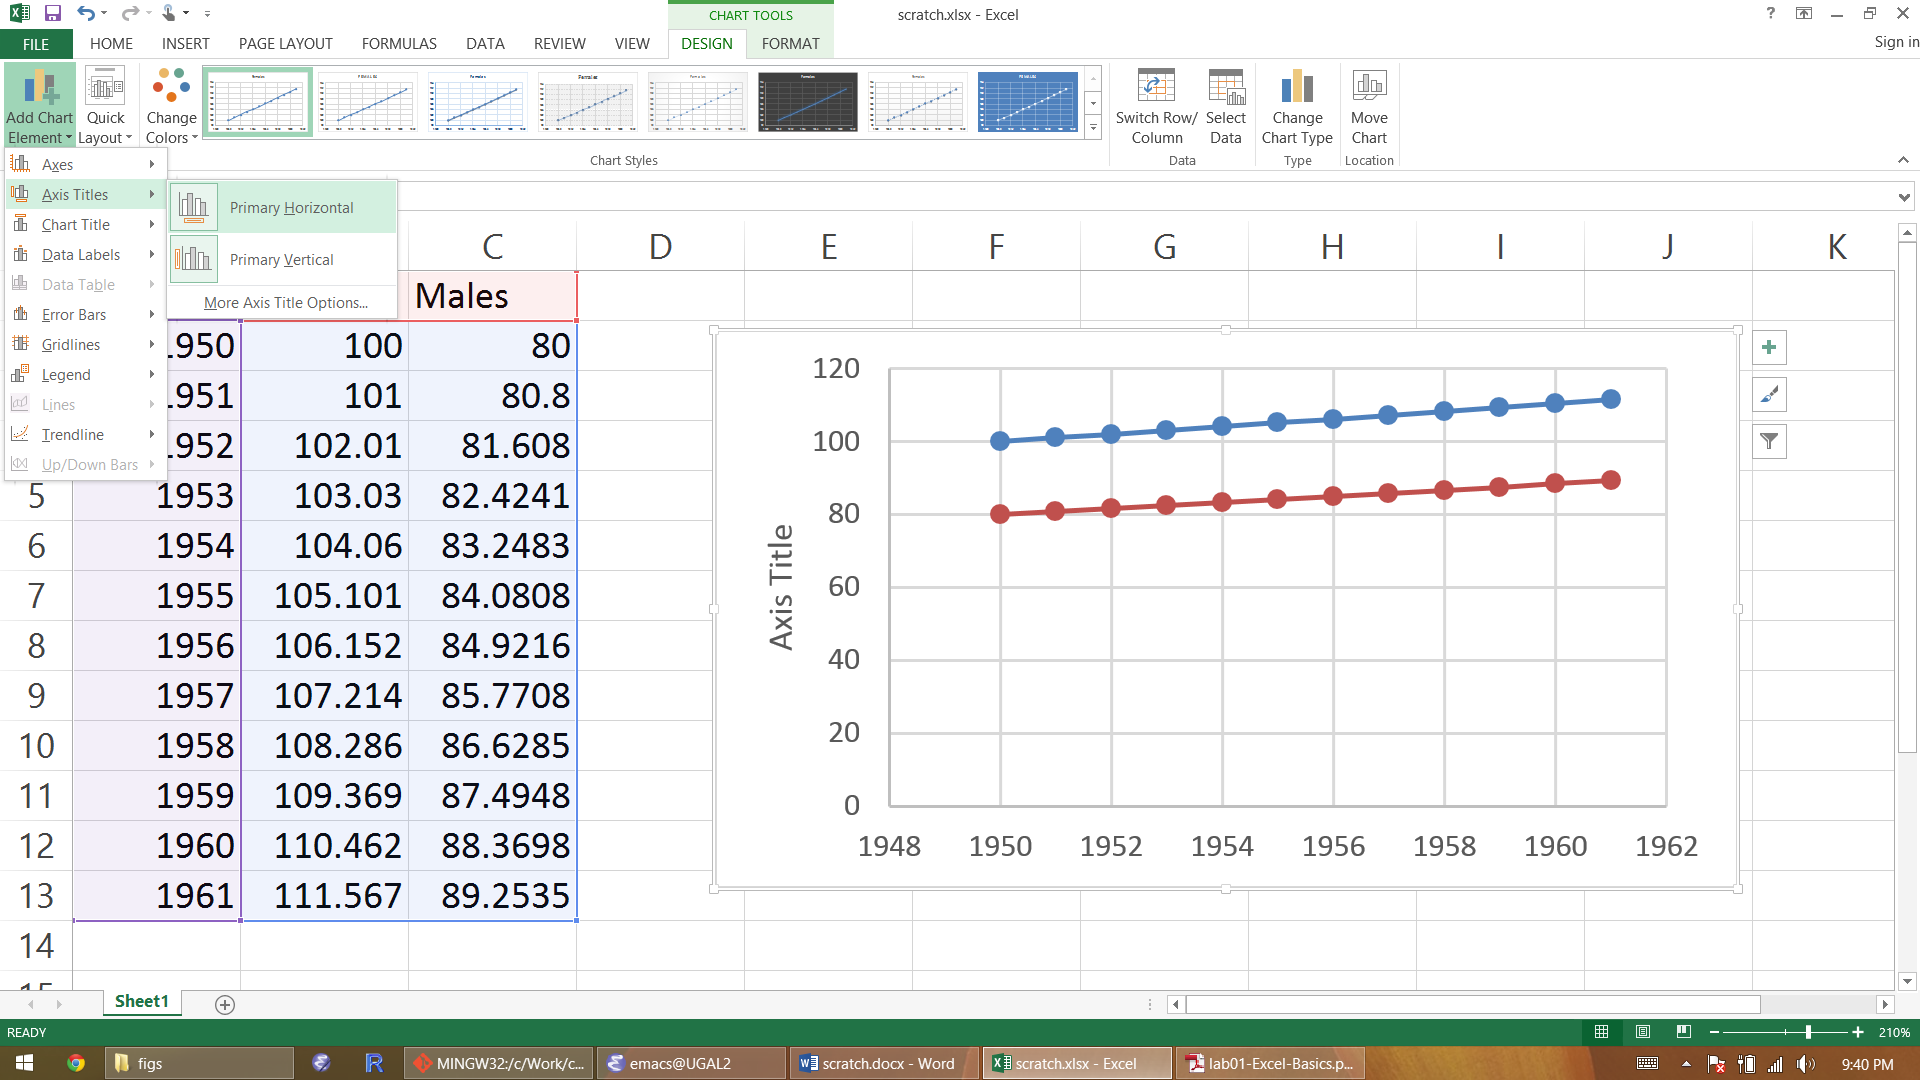
\includegraphics[width=\textwidth]{figs/customize2}}
    \begin{center}
      Add axis labels
    \end{center}
\end{frame}



\begin{frame}
  \frametitle{Customize}
    \fbox{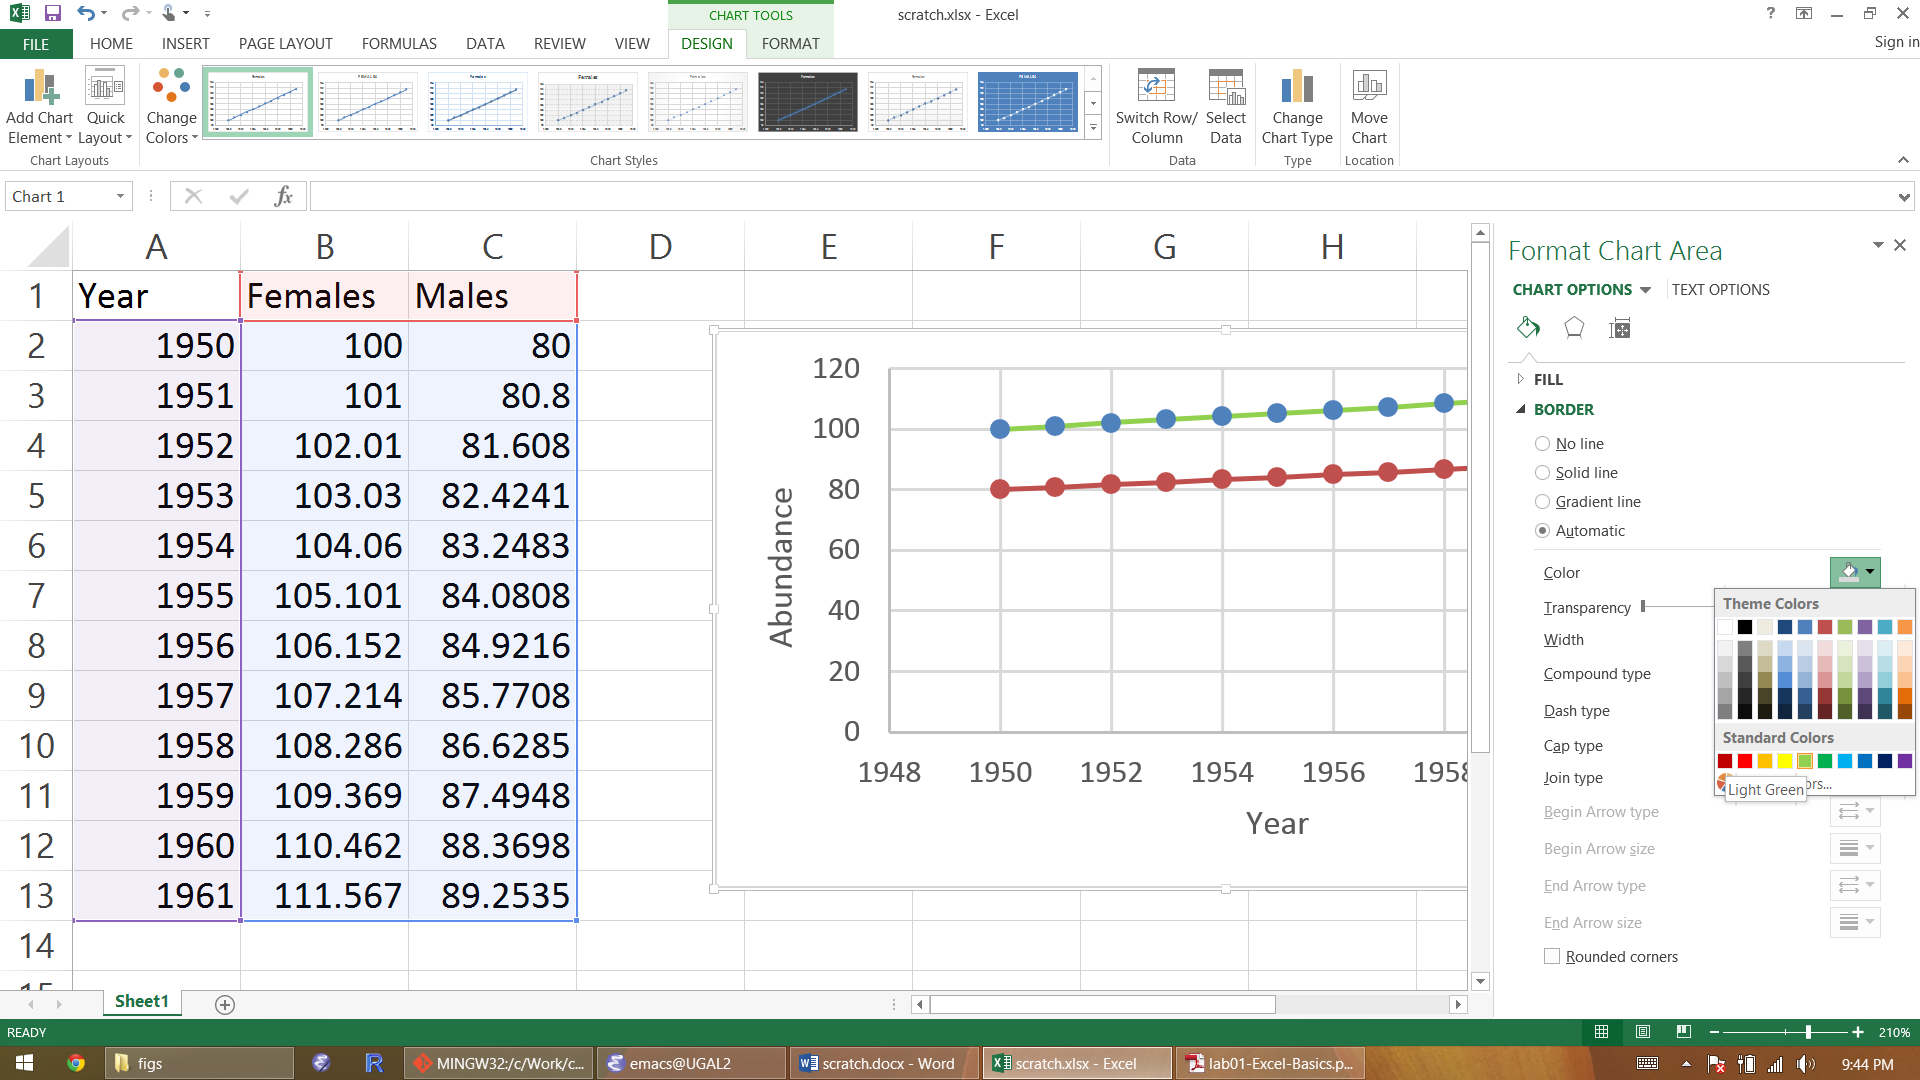
\includegraphics[width=\textwidth]{figs/customize3}}
    \begin{center}
      Change line color
    \end{center}
\end{frame}



\section{R}


\begin{frame}[fragile]
  \frametitle{R -- Software for statistical computing}
  {\bf R} can be downloaded here: \url{https://www.r-project.org/} \\
  \pause
  \vfill
  You can use the graphical user interface that comes with {\bf R}, or you
  can run {\bf R} through a system like {\bf ESS+emacs}
  (\url{https://vgoulet.act.ulaval.ca/en/home/}) or {\bf RStudio}
  (\url{https://www.rstudio.com/}) \\
  \pause
  \vfill
  Most people use {\bf RStudio} these days
\end{frame}


\begin{frame}
  \frametitle{RStudio}
  \fbox{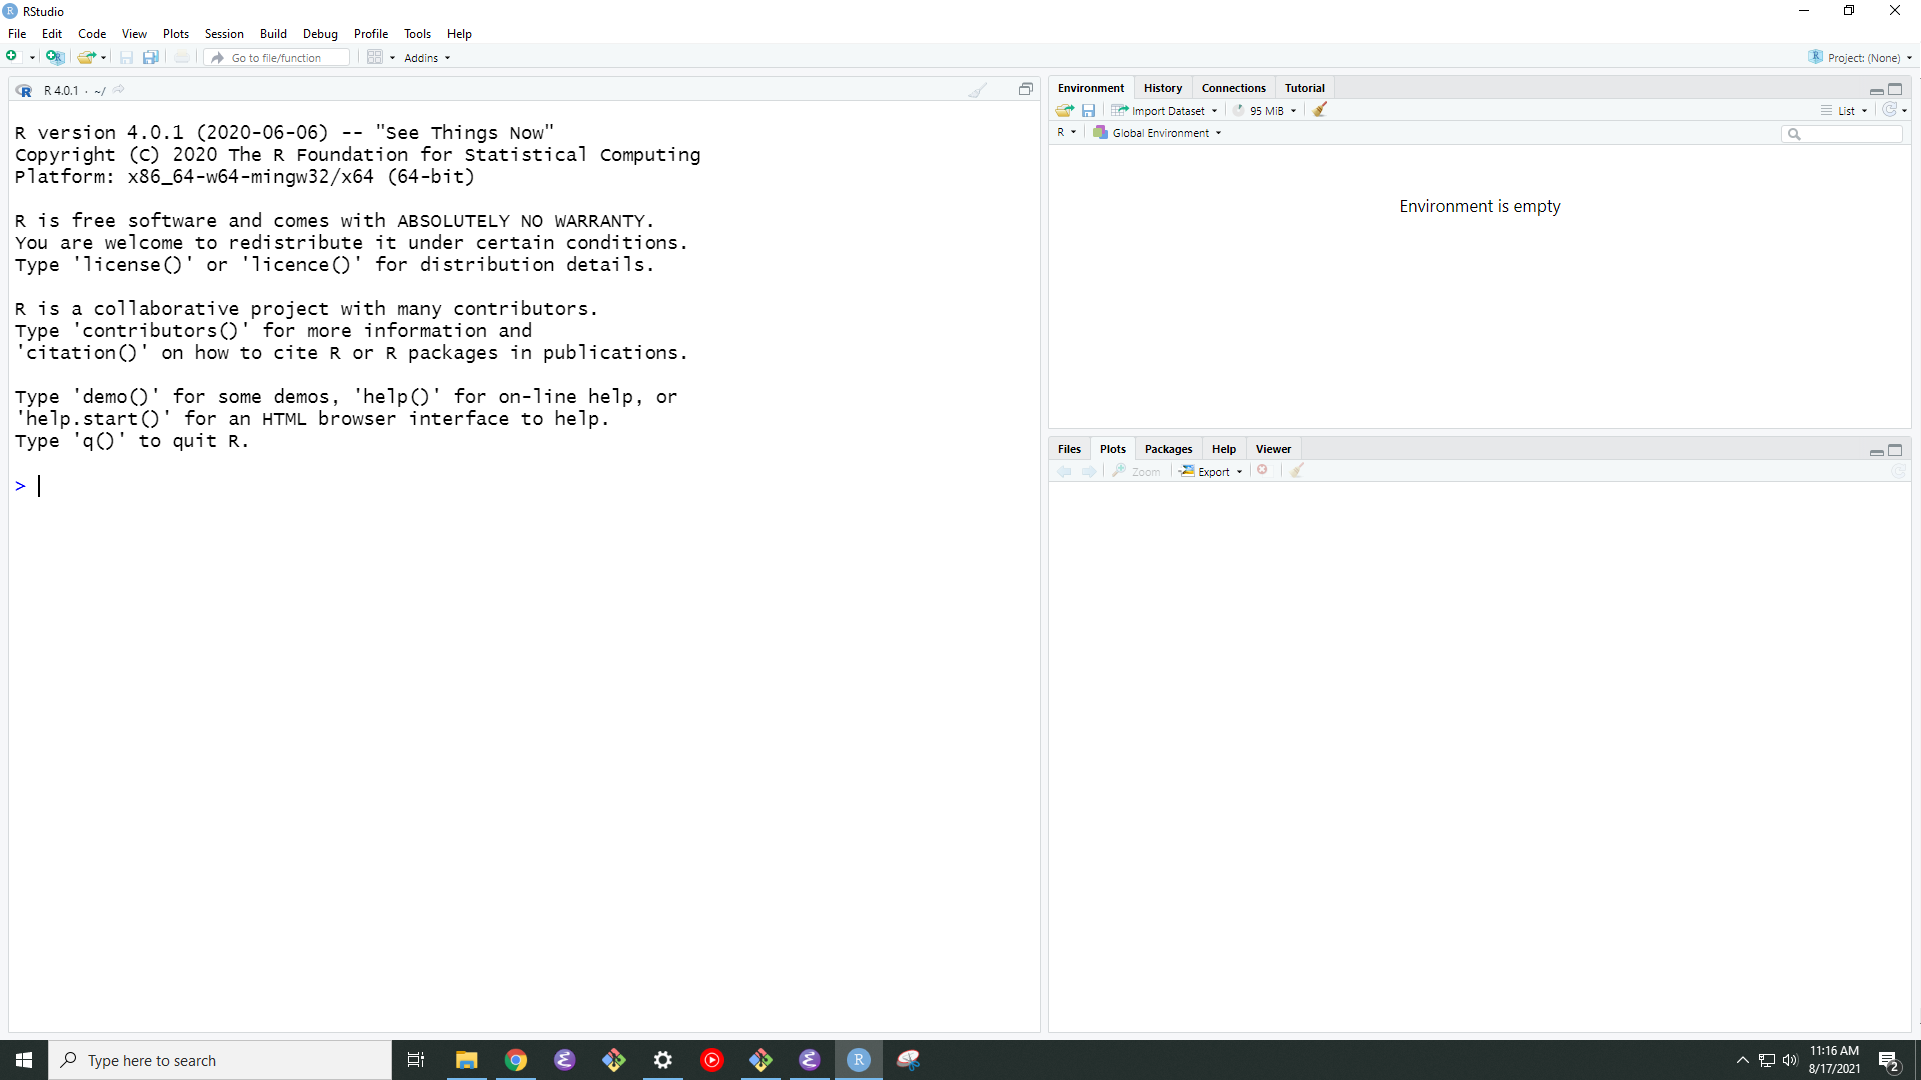
\includegraphics[width=\textwidth]{figs/rstudio-no-script}}
\end{frame}


\begin{frame}
  \frametitle{RStudio}
  To create a new script, click: {\tt File > New File > R Script} \\
  \fbox{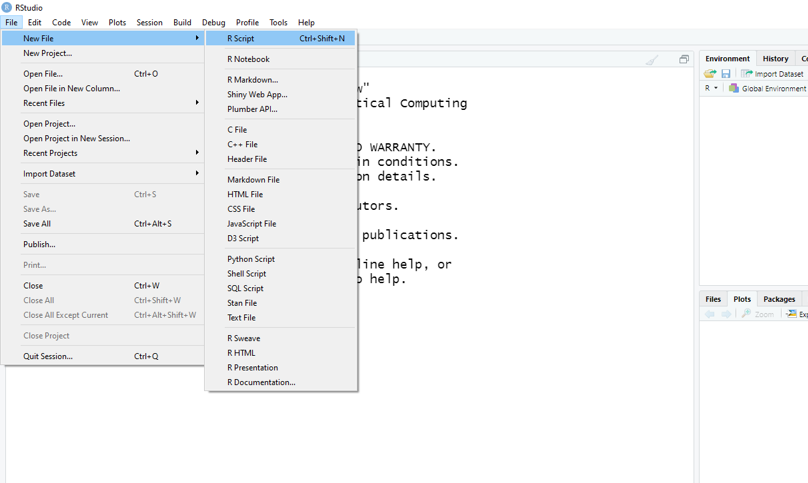
\includegraphics[width=\textwidth]{figs/rstudio-open-script}} \\
    Save your script using: {\tt File > Save As}
\end{frame}

\begin{frame}
  \frametitle{RStudio}
  \fbox{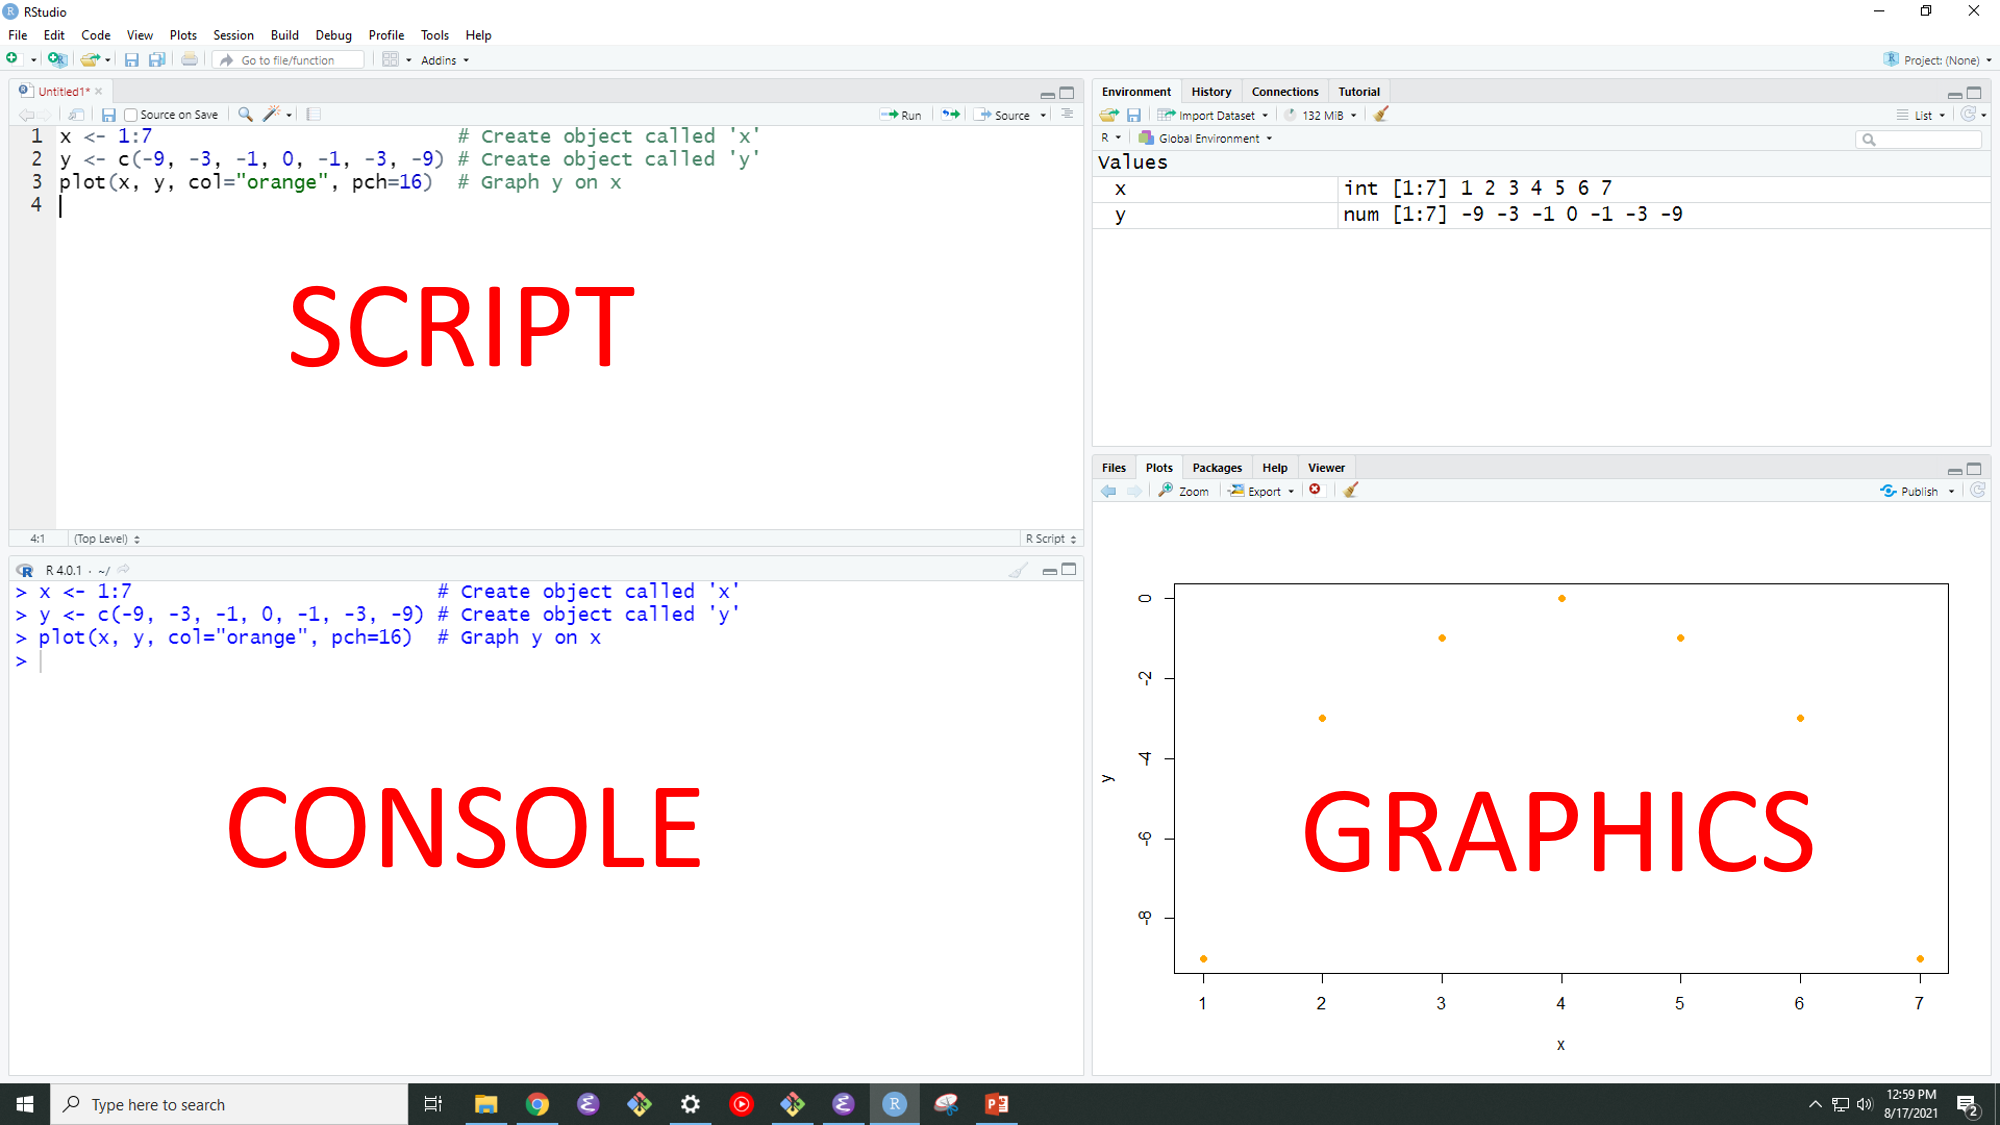
\includegraphics[width=\textwidth]{figs/rstudio-script-graphics}}
\end{frame}



\begin{frame}[fragile]
  \frametitle{Reproducing the Excel exercise}
  Create an object called \inr{year} to hold the sequence of years.
\begin{knitrout}\scriptsize
\definecolor{shadecolor}{rgb}{0.878, 0.918, 0.933}\color{fgcolor}\begin{kframe}
\begin{alltt}
\hlstd{year} \hlkwb{<-} \hlnum{1950}\hlopt{:}\hlnum{1961} \hlcom{# A vector of integers}
\hlstd{year}              \hlcom{# Type the name of an object to see its values}
\end{alltt}
\begin{verbatim}
##  [1] 1950 1951 1952 1953 1954 1955 1956 1957 1958 1959 1960 1961
\end{verbatim}
\end{kframe}
\end{knitrout}
\pause
\vfill
Use the \inr{length} function to determine the number of values in a
vector.
\begin{knitrout}\footnotesize
\definecolor{shadecolor}{rgb}{0.878, 0.918, 0.933}\color{fgcolor}\begin{kframe}
\begin{alltt}
\hlstd{nYears} \hlkwb{<-} \hlkwd{length}\hlstd{(year)}
\hlstd{nYears}
\end{alltt}
\begin{verbatim}
## [1] 12
\end{verbatim}
\end{kframe}
\end{knitrout}
\end{frame}


\begin{frame}[fragile]
  \frametitle{A simple population model}
  Create an empty vector to store the data on females. Set female
  abundance to 100 in the first year.
\begin{knitrout}
\definecolor{shadecolor}{rgb}{0.878, 0.918, 0.933}\color{fgcolor}\begin{kframe}
\begin{alltt}
\hlstd{females} \hlkwb{<-} \hlkwd{rep}\hlstd{(}\hlnum{NA}\hlstd{, nYears)}
\hlstd{females[}\hlnum{1}\hlstd{]} \hlkwb{<-} \hlnum{100}
\end{alltt}
\end{kframe}
\end{knitrout}
\pause
\vfill
Use a ``for loop'' to compute female abundance in subsequent years.
\begin{knitrout}
\definecolor{shadecolor}{rgb}{0.878, 0.918, 0.933}\color{fgcolor}\begin{kframe}
\begin{alltt}
\hlkwa{for}\hlstd{(t} \hlkwa{in} \hlnum{2}\hlopt{:}\hlstd{nYears) \{}
    \hlstd{females[t]} \hlkwb{<-} \hlstd{females[t}\hlopt{-}\hlnum{1}\hlstd{]} \hlopt{+} \hlstd{females[t}\hlopt{-}\hlnum{1}\hlstd{]}\hlopt{*}\hlnum{0.01}
\hlstd{\}}
\end{alltt}
\end{kframe}
\end{knitrout}
\pause
\vfill
\centering
\alert{\bf We will use ``for loops'' for almost every population model
  that we implement in R} \\
\end{frame}


\begin{frame}[fragile]
  \frametitle{A simple population model}
  \begin{columns}
    \begin{column}{0.41\textwidth}
      Generate the data on males using a single line of code.
\begin{knitrout}\footnotesize
\definecolor{shadecolor}{rgb}{0.878, 0.918, 0.933}\color{fgcolor}\begin{kframe}
\begin{alltt}
\hlstd{males} \hlkwb{<-} \hlstd{females}\hlopt{*}\hlnum{0.8}
\end{alltt}
\end{kframe}
\end{knitrout}
    \end{column}
\pause
    \begin{column}{0.58\textwidth}
      Put the objects in a \inr{data.frame}
\begin{knitrout}\scriptsize
\definecolor{shadecolor}{rgb}{0.878, 0.918, 0.933}\color{fgcolor}\begin{kframe}
\begin{alltt}
\hlstd{model1} \hlkwb{<-} \hlkwd{data.frame}\hlstd{(year, females, males)}
\hlstd{model1}
\end{alltt}
\begin{verbatim}
##    year  females    males
## 1  1950 100.0000 80.00000
## 2  1951 101.0000 80.80000
## 3  1952 102.0100 81.60800
## 4  1953 103.0301 82.42408
## 5  1954 104.0604 83.24832
## 6  1955 105.1010 84.08080
## 7  1956 106.1520 84.92161
## 8  1957 107.2135 85.77083
## 9  1958 108.2857 86.62854
## 10 1959 109.3685 87.49482
## 11 1960 110.4622 88.36977
## 12 1961 111.5668 89.25347
\end{verbatim}
\end{kframe}
\end{knitrout}
    \end{column}
  \end{columns}
\end{frame}


\begin{frame}[fragile]
  \frametitle{Graphics}
\begin{knitrout}\tiny
\definecolor{shadecolor}{rgb}{0.878, 0.918, 0.933}\color{fgcolor}\begin{kframe}
\begin{alltt}
\hlkwd{plot}\hlstd{(females} \hlopt{~} \hlstd{year,} \hlkwc{data}\hlstd{=model1,} \hlkwc{type}\hlstd{=}\hlstr{"o"}\hlstd{,} \hlkwc{xlab}\hlstd{=}\hlstr{"Year"}\hlstd{,} \hlkwc{ylab}\hlstd{=}\hlstr{"Abundance"}\hlstd{,}
     \hlkwc{lwd}\hlstd{=}\hlnum{2}\hlstd{,} \hlkwc{pch}\hlstd{=}\hlnum{16}\hlstd{,} \hlkwc{ylim}\hlstd{=}\hlkwd{c}\hlstd{(}\hlnum{0}\hlstd{,} \hlnum{120}\hlstd{))}
\hlkwd{lines}\hlstd{(males} \hlopt{~} \hlstd{year,} \hlkwc{data}\hlstd{=model1,} \hlkwc{type}\hlstd{=}\hlstr{"o"}\hlstd{,} \hlkwc{col}\hlstd{=}\hlstr{"blue"}\hlstd{,} \hlkwc{lwd}\hlstd{=}\hlnum{2}\hlstd{,} \hlkwc{pch}\hlstd{=}\hlnum{16}\hlstd{)}
\hlkwd{legend}\hlstd{(}\hlkwc{x}\hlstd{=}\hlnum{1950}\hlstd{,} \hlkwc{y}\hlstd{=}\hlnum{40}\hlstd{,} \hlkwc{legend}\hlstd{=}\hlkwd{c}\hlstd{(}\hlstr{"Females"}\hlstd{,} \hlstr{"Males"}\hlstd{),} \hlkwc{col}\hlstd{=}\hlkwd{c}\hlstd{(}\hlstr{"black"}\hlstd{,} \hlstr{"blue"}\hlstd{),} \hlkwc{lty}\hlstd{=}\hlnum{1}\hlstd{,} \hlkwc{pch}\hlstd{=}\hlnum{16}\hlstd{)}
\end{alltt}
\end{kframe}
\includegraphics[width=\maxwidth]{figure/plot-1} 
\end{knitrout}
\end{frame}




\begin{frame}
  \frametitle{Assignment}
  \small %\footnotesize
  \begin{enumerate}
    \item[1.] Create an Excel file and name it ``Yourlastname\_Yourfirstname''.
    \item[2.] Create the sheet shown on the next page using the techniques covered in this lab.
      \begin{itemize}
        \footnotesize
        \item Use auto-fill to create the first two columns.
        \item For the ``Adults'' column, use the equation shown
          for cells C3 through C22. Note: For cell C2, you can directly
          enter the value ``10''.
      \end{itemize}
    \item[3.] Copy ``Sheet1'' to a new sheet and change the color and
      thickness of the lines. You can pick any colors and thicknesses you want.
    \item[4.] Replicate steps 1--3 using a ``for
      loop'' in a self-contained {R} script.
    \item[5.] Upload the Excel workbook (with both sheets) and the
      R script to ELC.
  \end{enumerate}
\end{frame}


\begin{frame}
  \frametitle{Assignment}
  \fbox{\includegraphics[width=\textwidth]{figs/assignment-new}}
\end{frame}


\end{document}
